\chapter{Introduction}
\label{ch:Intro}

\par
The thesis will concern two topics of higher interest in current research. The first part of the thesis is on the Sachdev-Ye-Kitaev(SYK) model. The SYK model at its core is a model of a strongly interacting quantum dot with many flavors of electrons in it. Its rich solutions are targeted at explaining several unsolved problems in contemporary physics, including an elusive theory for the metallic phase of the cuprate high temperature  superconductors. 
The second part of the thesis will tackle the classic problem of the Kondo effect in a modern setting of strongly interacting electrons: Twisted bilayer graphene (TBG). 

\par 
As an artistic concept to which perhaps too much meaning should not be attached, we will see that underneath the description of both of these phenomena lies a hyperbolic geometry. In TBG, this will be identified in the hyperbolic Fermi surface contours. In the SYK model, the exotic physics will be described by the breaking of an emergent conformal symmetry, which can equivalently be described through the holographic duality by fluctuations of an Anti de-Sitter spacetime, which is the Lorentzian version of the Euclidean hyperbolic space.  

\newpage


\section{Fermions, Fermi surfaces and quasiparticles}

Condensed matter physics concerns the study of the quantum properties of matter. We know that solids are composed of atoms arranged in a crystalline structure. Their quantum description at its core is given by the many-body Schrodinger equation of all the electrons and ions that make up the solid, all interacting with each other. The first simplification one can make is to observe that the ions in a solid are composed of many protons and neutrons, and are much heavier than the electrons since $\nicefrac{m_p}{m_e} \approx 2000$. Then the solid's low energy dynamics can be modeled by the motion of free electrons and their interactions with each other through the electromagnetic force, and with the vibrations of the lattice, known as phonons~\cite{oppenheimer1927quantentheorie}. 

\par 
Schematically, in the language of second quantization, the Hamiltonian of the system of electrons can be written as 
\begin{align}
    H = \underbrace{\sum_k \epsilon_k c^\dagger_k c^{\phantom{\dagger}}_k}_{T} + \underbrace{\frac{g}{\Omega}\sum_{k,k^\prime,q} c^\dagger_{k+\frac{q}{2}}c^\dagger_{k^\prime -\frac{q}{2}}c^{\phantom{\dagger}}_k c^{\phantom{\dagger}}_{k^\prime}}_{V} \quad\quad, 
    \label{eq:schemHam}
\end{align}
where the kinetic and potential energy terms have been separated out. In Eq.~\eqref{eq:schemHam}, $\epsilon_k$ refers to the dispersion of bare electrons subject to the symmetry of the lattice, and $\Omega$ is the volume of the system under consideration. For simplicity, all interactions that the electrons are subject to are schematically represented by the constant $g$, which may come from their charged interactions or with phonons or impurities etc. In a real material, the interaction itself may have a long range (and hence a momentum dependence), or may even face retardation effects, but these are neglected for now. 

\par
Let's first consider the kinetic energy term, given by $T$, and let us also suppose the bare parabolic dispersion of free electrons in the Galilean continuum.
Just the fact that electrons are fermions obeying the Pauli exclusion principle means that the large density of free electrons in a metal each fill up the energy levels one by one, and the last few electrons to fill in would correspond to a gigantic energy scale. For example, in copper~\cite{Ashcroft1976} which has an electron density of $8.47\times 10^{28} m^{-3}$, the energy of the topmost occupied level turns out to be $7 eV$, which corresponds to about $81600 K$ in units of temperature. For reference, the surface of the sun is at a temperature of $5000 K$. 
\par 
This mammoth Fermi energy, which represents the magnitude of the kinetic energy in the total hamiltonian Eq.~\eqref{eq:schemHam},  is what is responsible in most cases to the success of Landau's Fermi liquid theory. Owing to the relative unimportance of the potential energy term, to lowest approximation, electrons can be considered to be completely non-interacting, from which weak interactions can be included perturbatively~\cite{luttinger1960ground,baym1961conservation,pines2018microscopic}. 
\par 
This can be understood mathematically using the language of Green's functions. Typically, the Green's function for free fermions has the defining feature of having a pole whenever the frequency matches the energy of an excitation:
\begin{equation}
        G^0(\vec{k},\omega) = \frac{1}{\omega + i\eta - \epsilon_{\vec{k}}} .
\end{equation}
The physically accessible information here is the spectral function, which is the negative imaginary part of the self energy. As a function of frequency, this has a delta function peak at $\omega = \epsilon_k$. 
\par
When interactions are included, the Green's functions pick up a self energy according to the Dyson's equation:
\begin{equation}
    G(\vec{k},\omega) = \frac{1}{\omega - \epsilon_{\vec{k}} - \Sigma(\vec{k},\omega)}
\end{equation}

The self-energy will have a frequency and momentum dependence, and also a real and an imaginary part. We can expand the self-energy around a vector on the Fermi surface, at low frequencies
\begin{equation}
    \Sigma(k,\omega) = \mathrm{const} + k\pdv{\Sigma(k,0)}{k}\eval_{k=k_F} + \omega\pdv{\Sigma(k_F,\omega)}{\omega}\eval_{\omega=0} + \cdots .
\end{equation}
We can use this to rewrite the Green's function in the form
\begin{align}
    G(k,\omega) &= \frac{1}{\omega\left(1 - \pdv{\Sigma}{\omega} \right) - \left(\epsilon_{\vec{k}} + k\pdv{\Sigma}{k}\right) + i\Gamma} \, , \nonumber \\ 
    &= \frac{Z}{\omega - \Tilde{\epsilon_{\vec{k}}} + i\Tilde{\Gamma}} \, , 
    \label{eq:FLGreensfunction}
\end{align}
where the quasiparticle residue is given by 
\begin{equation}
    Z = \left(1-\pdv{\Sigma(k_F,\omega)}{\omega}\eval_{\omega=0}\right)^{-1} .
\end{equation}
In this case, the spectral function which was a delta peak in the non-interacting case would just be shifted to the new position $\Tilde{\epsilon_{\vec{k}}}$, and would be a relatively sharp Lorentzian of width $\Tilde{\Gamma}$.

\par 
The success of Fermi liquid theory can be summarised succinctly by Eq.~\eqref{eq:FLGreensfunction}. The presence of weak interactions  serves to simply broaden the fermion spectral functions by a small amount compared to the Fermi energy, and leads to long lived quasiparticles. 

\par
When the Taylor series expansion is valid, i.e. the self energy is analytic ($\Sigma \sim \alpha + \beta\omega + \gamma\omega^2 + \cdots$), the quasi-particle residue would be finite. With the discussion so far, we see that quasiparticles exist ubiquitously in the low energy description of weakly interacting systems of fermions for this simple reason. 
\par 
However, this seems to not be the case in the normal state corresponding to a family of the cuprate high-Tc superconductors such as such as YBCO (YBa${}_2$Cu${}_3$O${}_{7-x}$), LSCO (La${}_{2-x}$Sr${}_x$CuO$_{}4$), and BSCCO(Bi${}_2$Sr${}_2$CaCu${}_2$O${}_{8+x}$) among others. These compounds are of immense practical value as they are the among highest temperature superconductors, whose superconducting transition temperature $T_c$ can be controlled by doping. The optimal doping where $T_c$ is the highest, their normal states above $T_c$ are characterized by an incoherent featureless spectral function at the antinodal directions indicating that there are no quasiparticles to be observed~\cite{keimer2015quantum,damascelli2003angle}. Furthermore, this state, dubbed a strange metal, does not follow any of the phenomenological predictions of Fermi liquid theory. It is characterized a plethora of exotic features, the most prominent of which is a linear in temperature resistivity starting from the highest temperatures, all the way down to the superconducting transition temperature, and further down until the lowest measurable temperatures if superconductivity is suppressed by a magnetic field~\cite{Zaanen2019}. There are also measured anomalies in the frequency scaling of its optical conductivity~\cite{marel2003quantum,michon2023reconciling} and magnetotransport~\cite{hussey2008phenomenology,ayres2021incoherent} among others. We are thus interested in scenarios where the simple quasiparticle picture might not hold in order to better understand these "non-fermi liquids". 
\par
In order to break quasiparticles down, we need at least one of two things to happen: either their lifetime must be much shorter than their mean energy (so they would decay quite quickly by scattering), or the quasiparticle residue corresponding to the pole must vanish. 
\par
At this point, one can mention a proposal from the past~\cite{varma1989phenomenology,ruckenstein1991theory,varma1993towards,varma2002singular}. The marginal or singular Fermi liquid, as the name suggests, is the most marginal way to create non-Fermi liquid behavior. Based on purely phenomenological terms, the linear term in the self energy is adjusted to include logarithmic corrections, which are weaker than the next leading (quadratic) term in the Taylor expansion. 
\par

The reason for doing this is as follows. If one supposes naively that the quasiparticle lifetime is the same as the scattering time that appears in the Drude model for electrical conductivity $\sigma = \frac{n e^2\tau}{m}$, with $\frac{1}{\tau} = \Tilde{\Gamma}$ according to Eq.~\eqref{eq:FLGreensfunction}, and that if one attributes the temperature dependence of the dc resistivity of the normal states of the cuprate high Tc superconductors  to a $T$-linear inverse quasiparticle lifetime $\Tilde{\Gamma}$ at zero frequency, then based on dimensional analysis, one can expect the imaginary part of the electron self energy to be linear in frequency at low temperature, i.e. $\Im\Sigma = \pi \omega $. Correspondingly from the Kramers-Kronig relations which are needed for reasons of causality, the real part of the self energy can be calculated to be~\cite{littlewood1991phenomenology}
\begin{equation}
    \Re\Sigma = \omega\log(\frac{\omega}{\omega_c}).
\end{equation}
\begin{figure}
    \centering
    \begin{subfigure}[b]{0.4\textwidth}
    \centering
    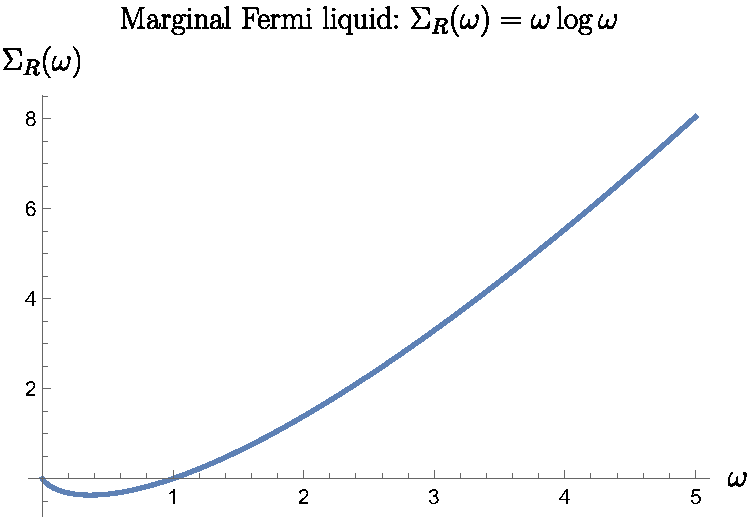
\includegraphics[width = \textwidth]{figures/introduction/MFLS.pdf}
    \end{subfigure}
    \begin{subfigure}[b]{0.4\textwidth}
    \centering
    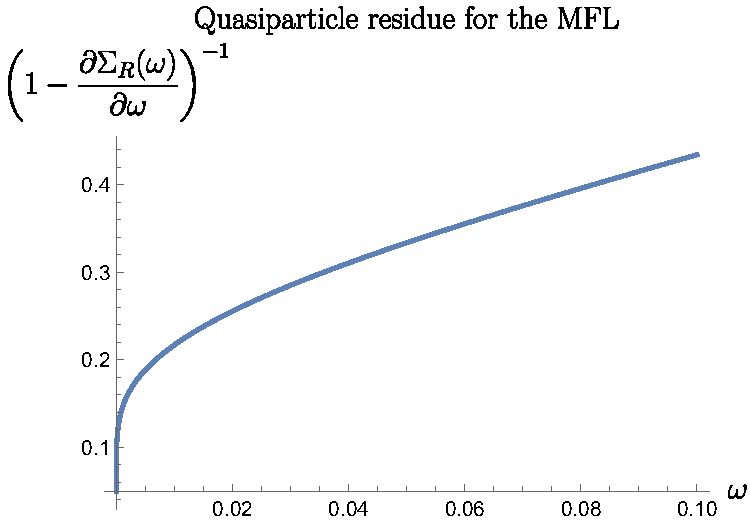
\includegraphics[width = \textwidth]{figures/introduction/MFLZ.pdf}
    \end{subfigure}
    \caption{Absence of quasiparticles in the marginal Fermi liquid.}
    \label{fig:MFLZ}
\end{figure}

\par
With this insight, we can understand the emergence of non-Fermi liquid behavior as a non-analytic behavior in the self energy, so that the quasiparticle residue vanishes, as seen from $\omega\rightarrow0$ of Fig.\ref{fig:MFLZ}. 
This simple (albeit naive) consideration  helps us understand why the linear in T resistance of cuprates cannot come from any quasiparticle description of the underlying electrons. Even if we try to fit a pole with the imaginary part that is needed for the correct decay rate, causality itself would render its residue to vanish.
The Green's function would now not have poles, but rather branch cuts on the $\omega$ axis. 
\par
The marginal Fermi liquid was constructed simply on phenomenological grounds, but it is of interest to construct some microscopic model which helps us understand the origin such a singular self energy.
Such an example is the SYK model, whose self energy, as we shall see goes as $\left|\omega\right|^{\nicefrac{1}{2}}$. It can be noted at this point that other examples of such power law self energies exist, such as near a quantum critical point in the Hertz-Millis theory of the ferromagnetic transition of itinerant electrons in a metal with $\Sigma \sim \omega^{2/3}$~\cite{Sachdev_2011}. 
\begin{figure}
    \centering
    \begin{subfigure}[b]{0.4\textwidth}
    \centering
    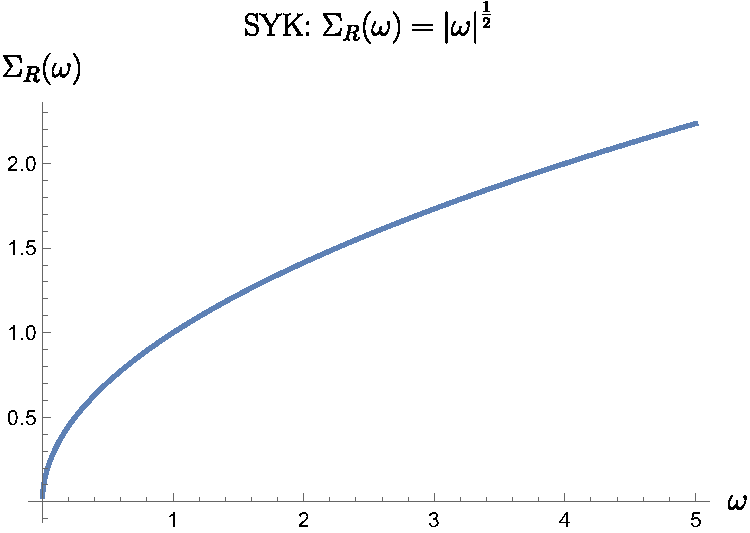
\includegraphics[width = \textwidth]{figures/introduction/SYKS.pdf}
    \end{subfigure}
    \begin{subfigure}[b]{0.4\textwidth}
    \centering
    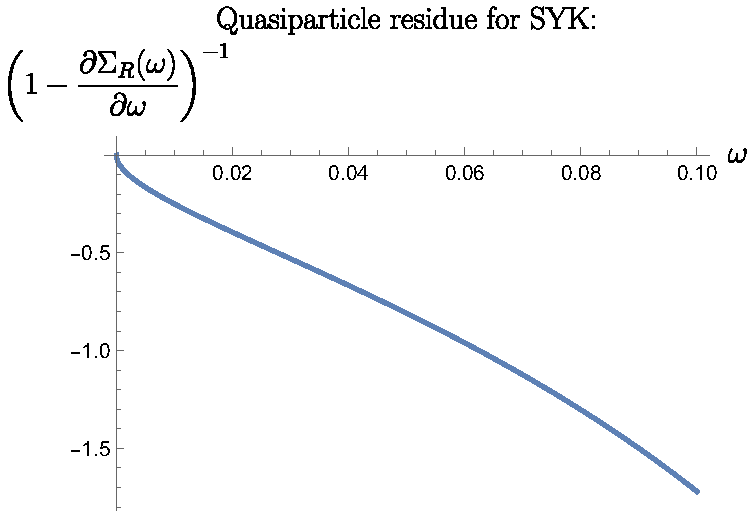
\includegraphics[width = \textwidth]{figures/introduction/SYKZ.pdf}
    \end{subfigure}
    \caption{Absence of quasiparticles in the SYK model.}
    \label{fig:SYKZ}
\end{figure}

\section{The SYK model}
The SYK model describes the physics of interacting fermions living on a strongly disordered quantum dot. Its simplest version can be constructed using a Hamiltonian of $N$ flavors of Majorana fermions interacting all-to-all with Gaussian random couplings. 
\begin{equation}
    H = \displaystyle \sum_{1\leq i<j<k<l\leq N} J_{ijkl}\,\psi_i\psi_j\psi_k\psi_l
\end{equation}
The random couplings are normally distributed, i.e 
\begin{align}
    \expval{J_{ijkl}} &= 0 \\
    \expval{J^2_{ijkl}} &= \frac{6 J^2}{N^3}.
\end{align}

\par
Henceforth, we will switch to Euclidean time (and imaginary frequencies). The free part of the Green's function is (with the normalization $\anticommutator{\psi_i}{\psi_j} = \delta_{ij}$)
\begin{align}
    G^0_{ij}(\tau) &= -\expval{\mathcal{T}\psi_i(\tau)\psi_j(0)} ,\nonumber\\
    &= -\frac{1}{2}\sgn(\tau) \, \delta_{ij}.
\end{align}
In Fourier space,  
\begin{align}
    G^0(\omega) = \int \dd\tau \,e^{i\omega\tau} G^0(\tau) = \frac{1}{i\omega}.
\end{align}

\subsection{The SYK self consistent equations}
We can now turn to look at the diagrams that dress the fermion Green's functions upon turning on interactions.  The disorder average enforces that the flavors of the four Majoranas at both the connecting vertices are identical, and simultaneously brings out a contribution $\sim \frac{J^2}{N^3}$ for each vertex pair. This means that in order for this diagram to not be suppressed in the large N limit, only diagrams which have three free intermediate lines summed over for each pair of vertices can survive. All these constraints 
 restrict the set of diagrams that survive at leading order in large $N$ to be just the melon diagrams shown in Fig.~\ref{fig:melons}, and the Green's function takes the form $G_{ij}(\tau) = G(\tau)\delta_{ij}$.

\par
With these considerations, the Dyson's equations can be represented as
\begin{figure}
    \centering
    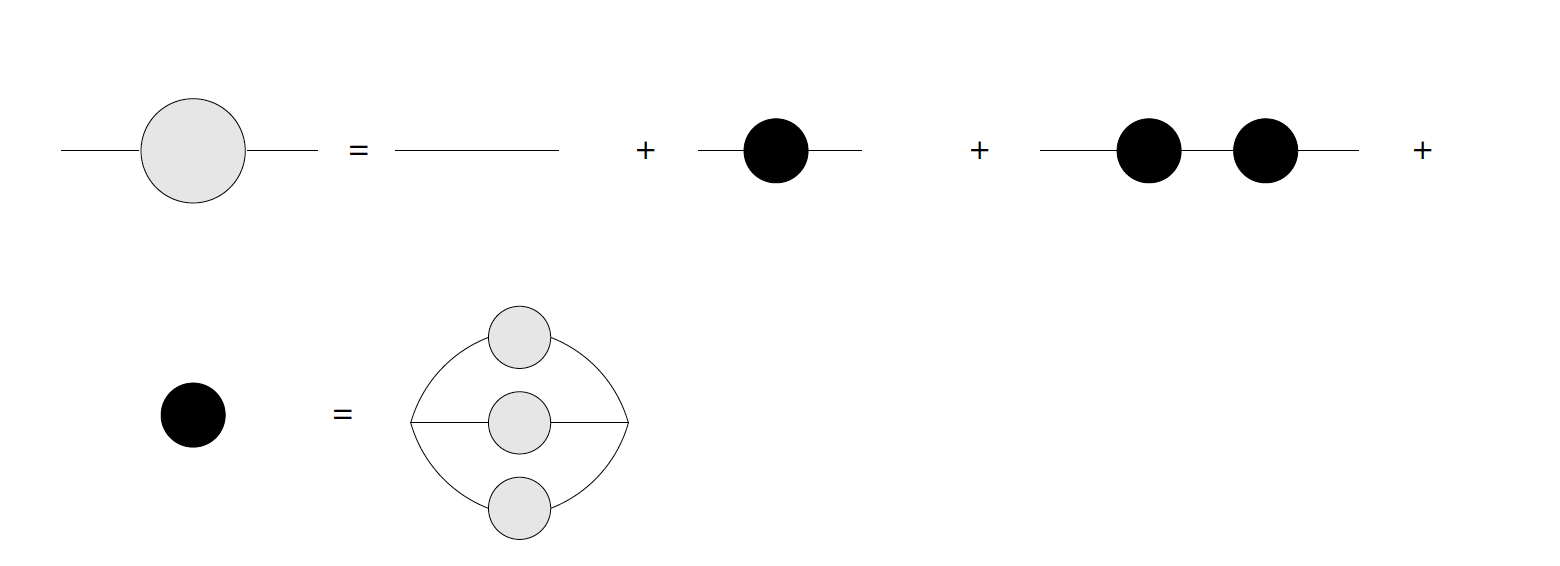
\includegraphics[width= \linewidth]{figures/introduction/Melons.png}
    \caption{Summing the Dyson series. Figure used from Ref.~\cite{maldacena_comments_2016}. The filled black dot represents the only self energy diagram that survives in the large $N$ limit.}
    \label{fig:melons}
\end{figure}
  
\par
This gives us the SYK equations: 
\begin{align}
    \left(G(\omega)\right)^{-1} = i\omega - \Sigma(\omega) \, ,\label{eq:sykeq1} \\ 
    \Sigma(\tau) = J^2\left(G(\tau)\right)^3 \,.\label{eq:sykeq2}
\end{align}
These are a set of equations that must be solved self-consistently: eq.(\ref{eq:sykeq1}) tells how the self-energy determines the Green's function, and eq.(\ref{eq:sykeq2}) says how the self-energy is set by the Green's function. 
They are not the most trivial to solve, since one is in real space, and the other in Fourier space. 
  

\par
The key to doing so is to assume that the self-energy dominates the free propagator's contribution at strong coupling in the IR $(\omega \xrightarrow{} 0)$.
Then, eq.(\ref{eq:sykeq1}) can be written as
\begin{equation}
    \int \dd\tau^\prime G(\tau,\tau^\prime)\Sigma(\tau^\prime,\tau^{\prime\prime}) = -\delta(\tau - \tau^{\prime\prime}) .
    \label{eq:confsykdyson}
\end{equation}
This is solved by the ansatz
\begin{equation}
    G_c(\tau) = \frac{b\sgn(\tau)}{\abs{\tau}^{2\Delta}} .
    \label{eq:Gc}
\end{equation}

% \subsection{SYK as an NCFT in the IR}
\par
Eq.~\eqref{eq:Gc} is the form of the Green's function of a conformal field theory (CFT), and commutes with all the generators of the conformal transformations in $0+1$ dimensions~\cite{schellekens1995conformal}. The scaling dimension $\Delta$ can be easily determined by a consistency condition that $\tau \xrightarrow{} b\tau$ should satisfy simultaneously Eq.~\eqref{eq:sykeq2}, (which would indicate that the self energy would need to scale as $\tau^{-6\Delta}$) and Eq.~\eqref{eq:confsykdyson}. 
\begin{align}
    b^{1 - 2\Delta - 6\Delta} &= b^{-1} ,\nonumber \\
    \implies \Delta &= \frac{1}{4} .
\end{align}
We can see again from simple dimensional analysis how the Green's function Eq.~\eqref{eq:Gc} scales as a function of frequency. The Fourier transformation
\begin{equation}
    \int_{-\infty}^\infty \dd\tau e^{i\omega\tau} \frac{\sgn(\tau)}{\abs{\tau}^{2\Delta}} \sim \abs{\omega}^{2\Delta-1},
\end{equation}
yields the branch-cut propagator result of $\Sigma(\omega)\sim \abs{\omega}^{\nicefrac{1}{2}} $, as promised, and we have with us a microscopic model for the breakdown of quasiparticles.  

\section{Other versions of the SYK used in this thesis}
It would be quite a fallacy to limit one's understanding of the physics of the SYK model to simply an artificial description of Majorana fermions in quantum dots - in fact, the original UV-completion of the SYK model was described by a random heisenberg coupled spin system~\cite{sachdev1993gapless}.
\par
Rather, its physical content  describes the emergence and the weak breaking of a new conformal symmetry in the infrared. In this section, we will describe some generalizations of the SYK model to include different kinds of degrees of freedom, which will be an emphasis of the fact that this class of models should be thought of as a description of a new IR fixed point. 

\subsection{Complex SYK}
The first generalization of the SYK fixed point that we will will consider is one that has a UV-completion that includes a conserved U(1) charge using complex fermions. This will be appropriately called the "complex-SYK" model~\cite{sachdev2015bekenstein,gu_notes_2020}. The hamiltonian will be written as 
\begin{align}
    H = \frac{1}{(2N)^{\nicefrac{3}{2}}}\displaystyle\sum_{ijkl = 1}^N\,J_{ij;kl}c^\dagger_ic^\dagger_jc^{\phantom{\dagger}}_kc^{\phantom{\dagger}}_l - \mu\sum_{i=1}^N c^\dagger_ic^{\phantom{\dagger}}_i \, .
\end{align}
In this UV hamiltonian, the total charge is simply given by 
\begin{align}
    Q = \frac{1}{N}\sum_i \expval{c^\dagger_i c^{\phantom{\dagger}}_i} .
    \label{eq:chargeUV_syk}
\end{align}
At $\mu = 0$, the model is at half filling, and $Q = \frac{1}{2}$ in this notation. 
\par
Similar to the Majorana SYK, this model also permits a conformally invariant IR, with exactly the same scaling dimension $\delta = \frac{1}{4}$. The infrared for the $\mu = 0$ case of the complex SYK model is indistinguishable from the Majorana SYK model in terms of the effective $G-\Sigma$ theory, in that the Green's functions are identical in the two cases. 
\par
At finite $\mu$, the effect of having a finite amount of charge is also indirectly felt by the infrared Green's functions, in the form of $G(\tau = 0^-) = Q$. This is shown in Fig.~\ref{fig:CSYKsolns} by the asymmetry between $\abs{G(\tau = 0^-)}$ and $\abs{G(\tau = 0^+)}$.
The Schwinger-Dyson equations in this case become~\cite{sachdev2015bekenstein}
\begin{subequations}
\begin{align}
    G(i\omega_n) &= \frac{1}{i\omega_n + \mu -\Sigma(\omega_n)} \\
    \Sigma(\tau) &= -J^2 G^2(\tau)G(-\tau)
    \label{eq:cSYKSDeqns}
\end{align}
\end{subequations}
For a solution of these equations to exist, one needs that $\Sigma(\omega_n \rightarrow 0) = \mu$, and at low energy and low temperatures it is solved by the same power law form. Then in that case, indeed one finds that there is a scaling solution to Eqs.~\eqref{eq:cSYKSDeqns} with the exponent $2\Delta - 1$, with $\Delta = \frac{1}{4}$ as before. 

\begin{figure}
    \centering
    \begin{subfigure}[t]{0.45\linewidth}
        \centering
        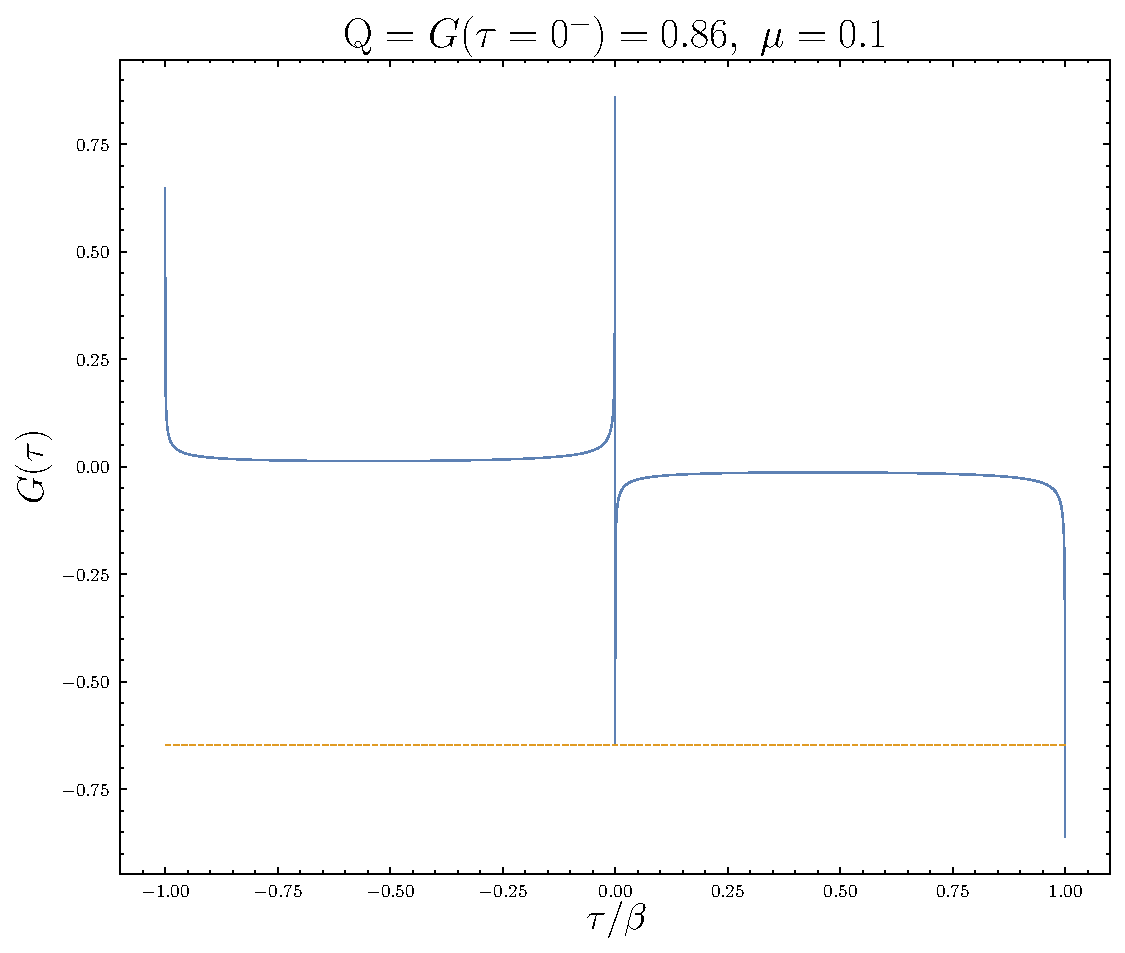
\includegraphics[width=\linewidth]{figures/introduction/Gtaushowingspectasymm.pdf}
    \end{subfigure}
    \begin{subfigure}[t]{0.45\linewidth}
        \centering
        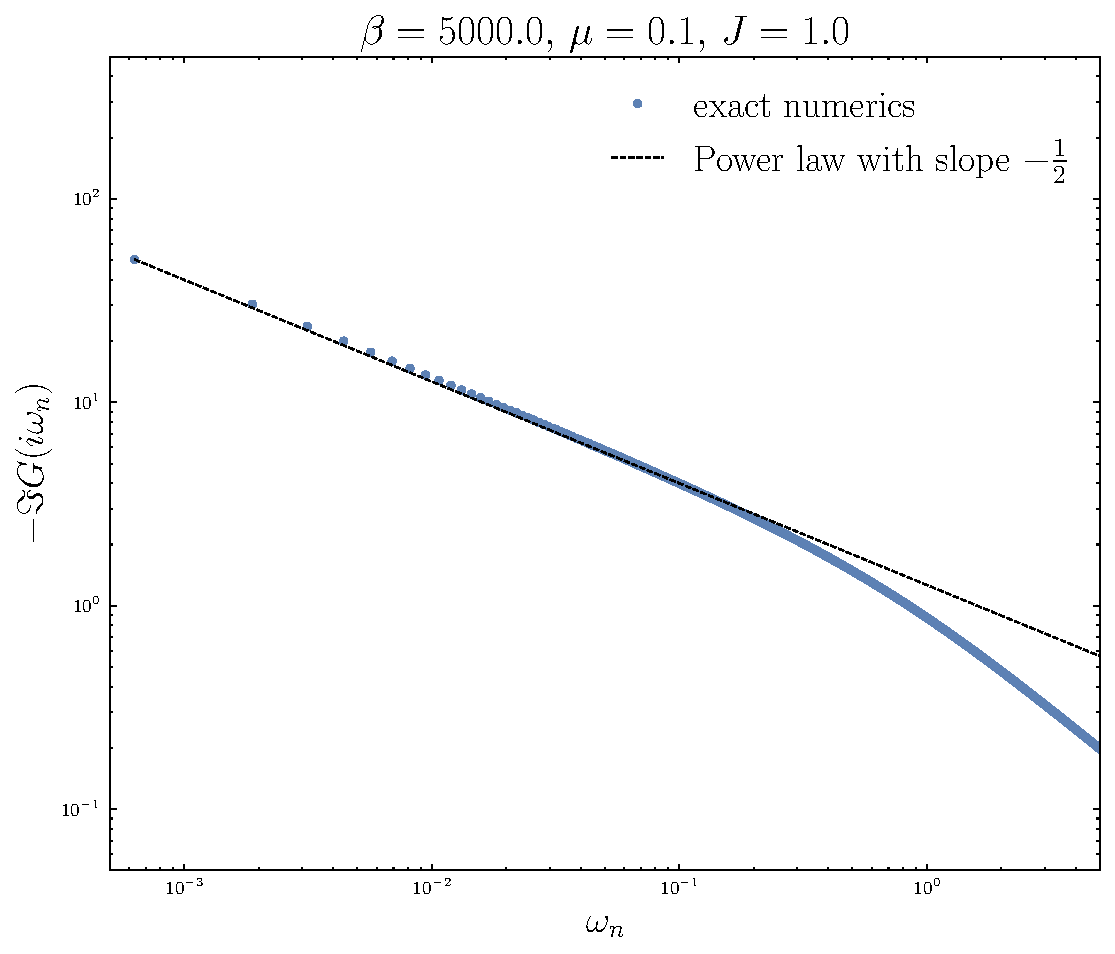
\includegraphics[width=\linewidth]{figures/introduction/complexSYKpowerlaw.pdf}
    \end{subfigure}
    \caption{Imaginary time solutions to the Schwinger-Dyson equations for the complex SYK model Eq.~\eqref{eq:SchDysEqnsYSYK_Imag}. Left: Asymmetry at $\tau=0$ in the case of a non-zero chemical potential, which measures the total charge. Right: Power law solution for $G(\omega_n)$ at low temperatures and low frequencies with the same scaling dimension as the Majorana SYK case, even with a finite chemical potential.}
    \label{fig:CSYKsolns}
\end{figure}



\subsection{Yukawa-SYK model}
The SYK model can also be generalized to include bosonic degrees of freedom. The Yukawa SYK (YSYK) model can be thought of as a zero dimensional analogue of the electron-phonon coupling Hamiltonian. This has been the subject of intense theoretical study in recent years~\cite{esterlis2019cooper,wang2020quantum,wang2020solvable,classen2021superconductivity,inkof2022quantum,pan2021yukawa,davis2023quantum,grunwald2024dynamical,choi2022pairing}. The model also allows for a generalization into higher dimension for a recently proposed universal theory of strange metals~\cite{patel2023universal,valentinis2023correlation,esterlis2021large,guo2022large,guo2023large,li2024strange} by being able to have a controlled large-N limit overcoming previous challenges~\cite{lee2009low}.

\par
The Hamiltonian for the Yukawa SYK is very reminiscent of the Fr\"ohlich or the Bardeen-Pines Hamiltonian for the electron-phonon interaction and can be written as 
\begin{equation}
    H_{Y-SYK} = -\mu\sum_{i=1}^N\sum_\sigma c^\dagger_{i,\sigma} c^{\phantom{\dagger}}_{i, \sigma} + \sum_{k=1}^M \frac{1}{2}\left(\pi_k^2 + \omega_0^2\phi_k^2\right) + \frac{\sqrt{2}}{N}\sum_{i,j,k}\sum_{\sigma}g_{ijk} c^\dagger_{i,\sigma} c^{\phantom{\dagger}}_{j,\sigma} \phi^{\phantom{\dagger}}_k .
    \label{eq:intrHYSYK}
\end{equation}
The are $N$ flavors of fermions, and $M$ flavors of bosons, and we are interested in the regime when both $N\rightarrow\infty, M\rightarrow\infty, \, \kappa = \frac{M}{N}$ held constant. 

\par
In the absence of time reversal symmetry, for the Hamiltonian to be hermitian, the couplings $g_{ij,k}$ have to satisfy 
\begin{equation}
    g_{ji,k} = g^*_{ij,k},
\end{equation}
and are drawn from the Gaussian unitary ensemble (GUE). At zero temperature, the low energy theory in this case is completely akin to the conventional SYK non-Fermi liquid, and develops an emergent conformal symmetry, with a scaling dimension set by $\kappa$. 
The Schwinger-Dyson equations in this case read
\begin{subequations}
\begin{align}
    \Sigma(\tau) &= \kappa \, g^2 \, G(\tau) D(\tau) \\
    \Pi(\tau) = &= -2g^2 \, G(\tau)G(-\tau) \\
    G(i\omega_n) &= \frac{1}{i\omega_n + \mu - \Sigma(i\omega_n)} \\
    D(i\nu_n) &= \frac{1}{\nu_n^2 + \omega_0^2 - \Pi(i\nu_n)} .
    \label{eq:SchDysEqnsYSYK_Imag}
\end{align}
\end{subequations}
The model is self-tuning to criticality~\cite{esterlis2019cooper}, i.e the bosons modes soften in the infrared. This is the condition that at zero temperature, $\Pi(\omega = 0) = \omega_0^2$.
In the infrared, we can obtain a non-Fermi liquid solution by making use of the zero-temperature conformal ansatz 
\begin{align}
    G(\tau) &= b\frac{\sgn(\tau)}{\abs{\tau}^{2\Delta_f}} ,\\
    D(\tau) &= d\frac{1}{\abs{\tau}^{2\Delta_b}} .
\end{align}
% These can be Fourier transformed using the identities
% \begin{align}
%         \int_{-\infty}^{\infty} d\tau\,\frac{\sgn(\tau)}{\abs{\tau}^\alpha} e^{i\omega\tau} &= i2^{1-\alpha}\sqrt{\pi}\frac{\Gamma(1-\frac{\alpha}{2})}{\Gamma(\frac{1}{2}+\frac{\alpha}{2})}\abs{\omega}^{\alpha-1}\sgn(\omega) , \\
%         \int_{-\infty}^{\infty} d\tau\,\frac{1}{\abs{\tau}^\alpha} e^{i\omega\tau}  &= 2^{1-\alpha}\sqrt{\pi}\frac{\Gamma(\frac{1}{2}-\frac{\alpha}{2})}{\Gamma(\frac{\alpha}{2})}\abs{\omega}^{\alpha-1}. 
% \end{align}
% We then get 
% \begin{align}
%     \Sigma(\omega) &= \kappa \, g^2 bd \, i2^{1-2(\Delta_f + \Delta_b)}\sqrt{\pi}\frac{\Gamma(1-(\Delta_f+\Delta_b))}{\Gamma(\frac{1}{2} + \Delta_f + \Delta_b)} \abs{\omega}^{2(\Delta_f+\Delta_b)-1}\sgn(\omega) \\
%     \Pi(\omega) &= 2g^2b^2 \, 2^{1-4\Delta_f}\sqrt{\pi} \frac{\Gamma(\frac{1}{2} - 2\Delta_f)}{\Gamma(2\Delta_f)}\abs{\omega}^{4\Delta_f-1}\\
%     G(\omega) &= b\,i2^{1-2\Delta_f}\sqrt{\pi}\frac{\Gamma(1-\Delta_f)}{\Gamma(\frac{1}{2}+\Delta_f)}\abs{\omega}^{2\Delta_f-1}\sgn(\omega) \\
%     D(\omega) &= d\,2^{1-2\Delta_b}\sqrt{\pi}\frac{\Gamma(\frac{1}{2}-\Delta_b)}{\Gamma(\Delta_b)} \abs{\omega}^{2\Delta_b-1}
%     \label{eq:scalingsolns}
% \end{align}
% The Dyson equation in the fully conformal limit, where the self energy wins over the free propagators are: (for now we work with $\mu = 0$ )
% \begin{align}
%      -1 &= G(\omega)\Sigma(\omega) \,, \\
%      -1 &= D(\omega)\Pi(\omega).
%     \label{eq:DysonFreq}
% \end{align}
% We see that in this case, only the product $b^2d$ is fixed in this fully conformal limit, and not separately the constants $b$ and $d$ themselves, as happens for regular SYK. However, this is an artifact of neglecting the short time, high frequency terms in the Dyson equation, and including the full UV corrections enables one to fix these constants, similar to the b-SYK model. The easy way to see this is that at short time, the free part of the Dyson equation should win over, and $G(\tau = 0^+)$ should be $-\frac{1}{2}\sgn(\tau)$, which is the fourier transform of $\frac{1}{i\omega}$.   

\par
% Eq.\eqref{eq:scalingsolns} and Eq.~\eqref{eq:DysonFreq} together imply that
% \begin{align}
%     2\Delta_f + \Delta_b &= 1 ,\\
%     \kappa \, \frac{\Gamma(1-\Delta_f)\Gamma(1-(\Delta_f+\Delta_b))}{\Gamma(\frac{1}{2}+\Delta_f)\Gamma(\frac{1}{2}+\Delta_f+\Delta_b)} &= -2 \frac{\Gamma(\frac{1}{2}-\Delta_b)\Gamma(\frac{1}{2}-2\Delta_f)}{\Gamma(\Delta_b)\Gamma(2\Delta_f)}.
% \end{align}
For $\kappa = 1$, we obtain the scaling dimensions $\Delta_f = 0.420374$, and $\Delta_b = 0.159252$.
\par 
At finite temperature, the model exhibits a rich phase diagram first outlined in Ref.~\cite{esterlis2019cooper}. For $g<1$, the highest temperatures are characterized by a limit of free fermions, where $G(\omega_n) \rightarrow \frac{1}{i\omega_n}$, and the low temperature phase is the finite temperature version of the non-Fermi liquid described above. The $g>1$ regime is characterized by a novel impurity like phase at intermediate and high temperature. This is shown pictorially in Fig.~\ref{fig:ESPhaseDiagram}.
\begin{figure}
    \centering
    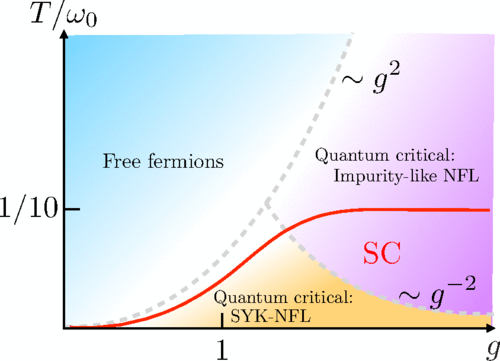
\includegraphics[width=0.7\linewidth]{figures/introduction/ESphasediag.png}
    \caption{Phase diagram of the Yukawa SYK model. Figure used from Ref.~\cite{esterlis2019cooper}.}
    \label{fig:ESPhaseDiagram}
\end{figure}

\par
In the presence of time reversal symmetry(TRS), the couplings in Eq.~\eqref{eq:intrHYSYK} are further constrained to be completely real, and $g_{ij,k}$ have to be drawn from the Gaussian orthogonal ensemble (GOE). This changes the ground state quite starkly, and the system is now described by a superconducting state. 
The reason for the reappearance of superconductivity on restoration of TRS can be most easily understood in analogy with the BCS case with $s-$ wave pairing. There, the electrons choose to pair with zero center of mass momentum, i.e. the state on the Fermi surface with momentum $\vec{k}$ pairs with its time reversal partner: the state with momentum $-\vec{k}$. The statement of TRS is that $E(\vec{k}) = E(-\vec{k})$, so both states required for pairing lie on the Fermi surface. It is obvious then that the breaking of TRS will lead to a reduction of phase space for pairing, and hence diminishing superconductivity.
\par
As an aside, another loose argument for this is that the broken time reversal symmetry can be thought of as introducing an artificial magnetic field, and the introduction of a magnetic field is the canonical way to suppress superconductivity.  
\par 
Coming back to the Yukawa SYK model, the restoration of TRS introduces a form of strong coupling superconductivity at low temperatures, and the equations of motion become the quantum critical Eliashberg equations~\cite{metlitski2015cooper,chubukov2020interplay,abanov2020interplay,she2009bcs}. This is a model of superconductivity betrothed to a quantum critical point, and is expected to be of importance in the study of the cuprate superconductors.
In this case, the non-Fermi liquid metallic phase becomes difficult to observe as it competes with the superconducting phase. The reason for this is that the temperature scale in which non-fermi liquid effects set in is parametrically the same as that at which superconductivity sets in, but however there might be a numerical prefactor which separates the two. However, one may interpolate between the TRS preserving and TRS breaking situations by linearly interpolating between the GOE and GUE ensembles, which has the effect of lowering $T_c$ from its maximum value. 
\par
In Chapter~\ref{chap:JosephsonWormhole} of this thesis, we will explore what happens when we couple two quantum critical superconductors through a weak link as is done conventionally~\cite{ambegaokar1963tunneling} and calculate the resulting Josephson current. We will see that this very coupling will be responsible for a wormhole-like state on the dual gravitational side.
 
\subsection{b-SYK}
\label{subsec:bSYK}
Given the importance of the SYK model, attempts have been made in order to realise it in an experimental situation. A comprehensive list of these attempts is provided in the recent review~\cite{chowdhury_sachdev-ye-kitaev_2021}. 

\par 
We will here first specifically mention Ref.~\cite{Chen2018} using graphene flakes (more will be said about graphene in Sec.~\ref{sec:graphene} below). It is well known in graphene that the presence of a strong magnetic field induces the formation of Landau levels, the lowest of which is pinned to zero energy. This completely flat band quenches the kinetic energy in Eq.~\ref{eq:schemHam}. The wavefunctions have non-trivial quantum geometry still and instead of being localized, are extended throughout the surface of the graphene. There is a zero mode generated for every quantum of flux that penetrates the sample, as is well known from the theory of the quantum hall effect. 

\par
The effects of the coulomb interaction projected onto the degenerate states of the flat band, next nearest neighbor hoppings and random onsite disorder all contribute to make the effective interactions seem almost completely random. 

\par
To provide evidence that the Hamiltonian thus generated is SYK like, the authors of  Ref.~\cite{Chen2018} took recourse to random matrix theory. They first calculated the coupling constants of the projected graphene Hamiltonian by explicit numerical diagonalization as a function of flux. They observed with increasing flux that as a new zero mode was added, the distribution of couplings changed random matrix universality class, in close analogy to the Altland-Zirnbauer classification for non-interacting Hamiltonians~\cite{altland1997nonstandard,fidkowski2010effects,fidkowski2011topological}, and this matches perfectly with the random matrix classes as a function of the number of fermions in the SYK model~\cite{garcia2016spectral,behrends2019tenfold,you2017sachdev}. 

\par 
A similar idea was used by Fremling and Fritz~\cite{fremling_bipartite_2021} to propose an experimental realization of a Majorana version of the SYK model. They consider the Kitaev honeycomb model of spins~\cite{kitaev2006anyons}, which is believed to be realized in many spin liquid candidates including the iridates like $\mathrm{Na}_2\mathrm{IrO}_3$, $\mathrm{H}_3\mathrm{Li}\mathrm{Ir}_2\mathrm{O}_6$ and more prominently in $\alpha-\mathrm{RuCl}_3$~\cite{trebst2022kitaev,banerjee2017neutron}. The low energy theory of the Kitaev honey comb model exhibits deconfinement of the spins into Majorana fermions. Fremling and Fritz noted that an analogue of a strong magnetic field creating flat Landau levels could be simulated by application of triaxial strain, and the remnant interactions in these materials, for instance the heisenberg interaction, projected onto these Majorana zero modes resulted in an SYK-like interaction.
\par
The catch, however, is that unlike the complex fermion case in the graphene flakes, these residual interactions are only non-vanishing for pairs of Majoranas on opposite sublattices of the bipartite honeycomb lattice(see Fig.\ref{fig:bsyk}). This leads to the emergence of the so-called bipartite SYK model (b-SYK), whose Hamiltonian is given by 
\begin{equation}
    H_{b-SYK} = \frac{1}{4}\sum_{i,j=1}^{N_A}\sum_{\alpha,\beta = 1}^{N_B} J_{ij\alpha\beta}\psi^A_i\psi^A_j\psi^B_\alpha\psi^B_{\beta}. 
    \label{eq:Hbsyk}
\end{equation}
Again, the couplings have some sense of Gaussianity: 
\begin{equation}
    \expval{J_{ij\alpha\beta}\,J_{i^\prime j^\prime \alpha^\prime \beta^\prime}} = \frac{J^2}{2\sqrt{N_A N_B}^3}\delta_{i,i^\prime}\delta_{j,j^\prime}\delta_{\alpha,\alpha^\prime}\delta_{\beta,\beta^\prime}
\end{equation}
Here, $N_A$ and $N_B$ are the number of sites in the $A-$ and $B-$ sublattice respectively, and need not be the same in a disordered system.
\par
Although the new model in eq.~\ref{eq:Hbsyk} contains only $\nicefrac{3}{8}$ of the non-zero couplings as the full all-to-all SYK model, it still shows an emergent conformal symmetry at low energy, with a different tunable conformal dimension for the Majoranas in each set~\cite{Fremling_2022}. Such generalizations of the SYK model created by repeated pruning of the fully connected graph of couplings falls into the family of the so called "sparse SYK" models~\cite{xu_sparse_2020,garcia-garcia_sparse_2021,caceres2021sparse,caceres2023out}.

\begin{figure}
    \centering
    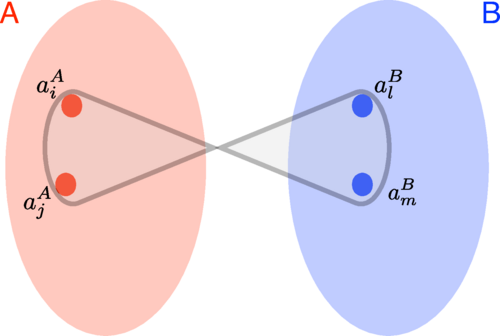
\includegraphics[scale = 0.5]{figures/introduction/bSYK.png}
    \caption{Schematic of the b-SYK model. There are 2 sets of Majorana fermions living on each of the two bipartite lattices of the honeycomb lattice. The interactions of the model are such that the Majoranas do not interact within a set, but every pair of Majorana degrees of freedom in each set interacts with a Gaussian random coupling with every pair of Majoranas on the other set. Figure from Ref.~\cite{Fremling_2022}.}
    \label{fig:bsyk}
\end{figure}



\section{Holographic dual of the SYK model and $N-AdS_2$ spacetime}
% This emergent conformal symmetry in the deep infrared is weakly broken by the free propagator $i\omega$ term in the Dyson equation Eq.~\eqref{eq:sykeq1}. The sub-leading to conformal corrections can be computed by an expansion of the action about the conformal saddle point, and can be shown in zero temperature to be of the form~\cite{maldacena_comments_2016}
% \begin{equation}
%     G(\tau) = G_c(\tau)\left(1-\frac{1}{\sqrt{2}J}\frac{1}{\abs{\tau}} + \cdots \right).
% \end{equation}
The correct path integral representation of the SYK effective action is given in terms of a two-time formalism, and the time-translation invariant solution Eq.\eqref{eq:Gc} only represents the classical saddle. The disorder averaged path integral can be written as
\begin{align}
    S = -\log\det\left(\partial_\tau + \Sigma(\tau,\tau^\prime)\right) - \int d\tau d\tau^\prime G(\tau,\tau^\prime)\Sigma(\tau,\tau^\prime) + \frac{J^2}{4} G(\tau,\tau^\prime)^4.
\end{align}
Without imposing time-translation symmetry, the saddle point equations would be Eq.~\eqref{eq:confsykdyson} and the self energy equation Eq.~\eqref{eq:sykeq2} rewritten to be
\begin{equation}
    \Sigma(\tau,\tau^\prime) = J^2\,\left[G(\tau,\tau^\prime)\right]^3. 
    \label{eq:twotimesykeq2}
\end{equation}

\par
It was observed that these set of equations in the fully conformal limit possessed an additional emergent symmetry of time reparametrizations~\cite{kitaev2018soft,maldacena_comments_2016,sachdev2015bekenstein}. 
This means that for every solution $G(\tau,\tau^\prime), \Sigma(\tau,\tau^\prime)$ that solves Eqs.~\eqref{eq:confsykdyson} and \eqref{eq:twotimesykeq2}, one can get yet another solution by picking an arbitrary function $f(\sigma)$ to obtain another function pair of functions $\Tilde{G}(\sigma,\sigma^\prime), \Tilde{\Sigma}(\sigma,\sigma^\prime)$ such that 
\begin{align}
    G(\tau,\tau^\prime) &= \frac{1}{\abs{f^\prime(\sigma)f^\prime(\sigma^\prime)}^\Delta}\Tilde{G}(\sigma,\sigma^\prime) \\
    \Sigma(\tau,\tau^\prime) &= \frac{1}{\abs{f^\prime(\sigma)f^\prime(\sigma^\prime)}^{1-\Delta}}\Tilde{\Sigma}(\sigma,\sigma^\prime)
    \label{eq:repatsymm}
\end{align}
that also satisfies the same equations Eqs.~\eqref{eq:confsykdyson} and \eqref{eq:twotimesykeq2}. 
\par
It turns out that starting from the conformal solution Eq.~\eqref{eq:Gc} 
\begin{equation}
    G_c(\tau,\tau^\prime) = b \frac{\sgn(\tau-\tau^\prime)}{\abs{\tau-\tau^\prime}}^{2\Delta},
\end{equation}
and picking a function from the $\mathrm{SL}(2,\mathrm{R})$ group i.e. $\tau = f(\sigma) = \frac{a\sigma + b}{c\sigma + d}$ with $ad-bc = 1$, leaves the saddle point solution invariant, i.e. $G_c(\tau,\tau^\prime) = \Tilde{G}_c(\sigma,\sigma^\prime)$. 

\par
For any other choice of the function $f$, we get new solutions to the saddle point equations , in fact infinitely many of them. This is an artifact of the far infrared limit, and the physical solution is determined by the function that minimizes the UV $i\omega$ term that has been neglected in the full action. This turns out to be the zero temperature scaling solution that we have written down. This is a motivation for an effective field theory for fluctuations around the SYK far infrared conformal fixed point - we simply write down an action with the fewest number of derivatives that vanishes for $f(\tau)$ in the $\mathrm{SL}(2,\mathrm{R})$ group. This is termed the Schwarzian action~\cite{maldacena_comments_2016, kitaev2018soft}
\begin{equation}
    S = \alpha_s \int d\tau \, \{f(\tau),\tau\}, \quad  \{f(\tau),\tau\} = \frac{f^{\prime\prime\prime}}{f^\prime} - \frac{3}{2}\left(\frac{f^{\prime\prime}}{f^\prime}\right)^2, 
    \label{eq:SchwActionDefn}
\end{equation}
and is the correct low energy theory of the breaking of conformal symmetry in the SYK model. The constant $\alpha_s$ in front is non-universal and can be fixed from either thermodynamics or the numerical evaluation of the four point function in the full UV-complete theory. 

We will consider one special choice of time reparametrization: $\tau = f(\sigma) = \tan{\frac{\pi\sigma}{\beta}}$. Written in this way, it is clear that the coordinate $\sigma$ represents a circle from $0$ to $\beta$ in imaginary time. Hence the propagator that we must obtain on using this in Eq.~\eqref{eq:repatsymm} should represent the Green's function of the IR limit of the SYK model when it is put at a finite temperature $\beta$. Doing the algebra, we see that 
\begin{align}
    \Tilde{G}(\sigma,\sigma^\prime) &= \left(\frac{\pi}{\beta}\right)^2 \left(\sec(\frac{\pi\sigma}{\beta})\sec(\frac{\pi\sigma^\prime}{\beta})\right)^{2\Delta} b \frac{\sgn(\sigma-\sigma^\prime)}{\abs{\tan(\frac{\pi\sigma}{\beta})-\tan(\frac{\pi\sigma^\prime}{\beta})}^{2\Delta}}  \nonumber \\
    &= b \frac{\sgn(\sigma-\sigma^\prime)}{\abs{\frac{\pi}{\beta}\sin(\frac{\pi}{\beta}(\sigma-\sigma^\prime))}^{2\Delta}}, 
\end{align}
where we used in the last step that $\cos x \cos y (\tan x - \tan y ) = \sin x\cos y - \cos x \sin y  = \sin (x - y)$. 
This particular choice of the function $f$ is not in the $\mathrm{SL}(2,\mathrm{R})$ group, and will contribute non-trivially to the action in eq.~\eqref{eq:SchwActionDefn}. The Schwarzian derivative itself for this case can be calculated to be $\frac{2\pi^2}{\beta^2}$, and that is equal to the finite temperature correction to the free energy. This directly implies that the low temperature entropy will be of the linear Sommerfeld form. 
\par
There is a remarkable connection between SYK systems and black holes in general relativity though a holographic duality. In some aspects, the behavior of the two parallel each other. The rest of this section is dedicated to explaining how this can be.
\par
The Schwarzian action is also the minimal action that describes the propagation of a boundary graviton in a 2 dimensional nearly Anti de Sitter spacetime ($N$-$AdS_2)$~\cite{maldacena2016conformal,chowdhury_sachdev-ye-kitaev_2021}. The reasoning is the following. In Euclidean signature, this is just a hyperbolic space with the metric 
\begin{equation}
    ds^2 = \frac{dt^2 + dz^2}{z^2}. 
    \label{eq:ads2metric}
\end{equation}
When one wants to study a finite part of the space, we want to cut it off along a boundary curve specified by $t(u), z(u)$, where the affine parameter $u$ is a local time coordinate on this curve. Staying $\epsilon$ away from the boundary at $z=0$ of and studying only curves of a fixed length, leaves still a choice of $t(u)$ being arbitrary, and different choices should correspond to different boundary curves. However, $AdS_2$ being a maximally symmetric space has $\mathrm{SL}(2,\mathrm{R})$ as an isometry, and different curves generated by 
\begin{equation}
    \Tilde{t}(u) = \frac{a t(u) + b}{c t(u) + d}, \quad ad-bc = 1.
    \label{eq:SL2Rgravity}
\end{equation}
all map on to each other, and other choices of reparametrizations of $t(u)$ correspond to fluctuations of the boundary spacetime, hence describing a boundary graviton. 

\par
It turns out that just simple $AdS_2$ spacetime is non-dynamical, in that the Einstein-Hilbert action is identically zero for all metric configurations since gravity in two dimensions is topological. To have a meaningful gravity theory, one needs to look at nearly $AdS_2$ or $N-AdS_2$ spaces, which are described by dilatonic theories of gravity, called the Jackiw-Teitelboim (JT) gravity~\cite{almheiri2015models, sarosi2017ads} with the action 
\begin{equation}
    S = -\frac{1}{16\pi G}\left[\int d^2 x \, \phi\sqrt{g} (R + 2) + 2\int_{\partial M} \phi_b K\right] 
\end{equation}
with a dynamical dilaton field $\phi$ that acts as an effective Newton's constant. 

\par
From similar arguments made for the SYK case, with the reparametrization symmetry acting in this case as eq.~\eqref{eq:SL2Rgravity}, the low energy effective action describing the propagation of the boundary graviton of this nearly $AdS_2$ space will once again be exactly the Schwarzian action. 
\par
We will take a moment to show how an $N$-$AdS_2$ space can come from a reduction from a higher dimensional space. In the process, we will uncover intuition for the role played by black holes in $AdS_2$ in regards to their dual field theories being at finite temperature.
\par
According to the holographic duality~\cite{maldacena1999large,gubser1998gauge,witten1998anti,zaanen2015holographic}, there is a dictionary that maps conformal field theories to spacetime geometries. The precise statement of this duality is that the partition functions of the boundary CFT and the bulk geometry are equal to each other. When we want to describe the  boundary theory at a finite temperature, it has to it an associated entropy, simply from the fundamental laws of thermodynamics. The empty AdS metric described in Eq.~\eqref{eq:ads2metric} does not have any entropy at all. Its is known from the work of Bekenstein~\cite{bekenstein1973black}, that the only what that spacetime geometry can have either an entropy or a temperature is if it had a black hole in it. The entropy then is proportional to the area of the black hole's event horizon, and the temperature is given by the Hawking temperature. 
\par 
We shall briefly sketch how this works in practice by considering an explicit  example~\cite{sachdev2015bekenstein,faulkner2011emergent,faulkner2011holographic}. Let us consider the Reissner-Nordstrom(RN) metric for planar black holes in asymptotic $AdS_{d+2}$. 
The metric from the solutions of Einstein's equations is given by
\begin{align}
    ds^2 = \frac{r^2}{R^2}\left(-f dt^2 + d\vec{x}^2\right) + \frac{R^2}{r^2}\frac{dr^2}{f}, 
    \label{eq:RNmetric}
\end{align}
where $R$ is the radius of $AdS_{d+2}$, and with the emblackening factor 
\begin{align}
    f = 1+\frac{\Theta^2}{r^{2d}} - \left(r_0^{d+1} + \frac{\Theta^2}{r_0^{d-1}}\right)\frac{1}{r^{d+1}}\,.
    \label{eq:RNemblackening}
\end{align}
The quantity $\Theta$ is proportional to the charge in the boundary theory, but we will not write it explicitly here for simplicity, for our current purposes we can just treat it as a constant. The black hole horizon is where the metric component $g_{tt}$ vanishes, and hence $f = 0$ implies that the horizon is at $r = r_0$ in these coordinates. 
\par
The Hawking temperature is determined by the surface gravity, which is the amount of acceleration a body needs to be at rest just near the horizon. For this Reissner Nordstrom metric in Eq.~\ref{eq:RNmetric}, it is given by~\cite{sachdev2015bekenstein,faulkner2011emergent}
\begin{align}
    T = \frac{(d+1)r_0}{4\pi R^2}\left(1 - \frac{(d-1)\Theta^2}{(d+1)r_0^{2d}}\right) \, .
\end{align}
We can observe that the Hawking temperature is zero when the horizon is at a position $r_0 = r_\ast$, such that 
\begin{align}
    \Theta^2 = \frac{d+1}{d-1} r_\star^{2d} \, .
\end{align}
At exactly this location of the horizon, we can look at the near horizon limit of Eq.~\eqref{eq:RNemblackening}, buy expanding 
\begin{align}
    r = r_* + \frac{1}{\zeta}
\end{align}
for leading order in $\zeta$. The metric that we arrive at then is 
\begin{align}
    ds^2 = \underbrace{R_2^2\frac{-dt^2 + d\zeta^2}{\zeta^2}}_{AdS_2} + \underbrace{\frac{r_\ast^2 d\vec{x^2}}{R^2}}_{\mathbb{R}^d} \, ,
    \label{eq:zerotempAds2}
\end{align}
and we see that the metric has factorized into $AdS_2 \times R^d$. We have also expressed an effective $AdS_2$ radius in terms of the radius of the full $AdS_{d+2}$ space as $R_2^2 = \frac{R^2}{d(d+1)}$. This can be compared with Eq.~\ref{eq:ads2metric}, only here we have the Minkowski signature.
\par
When the position of the horizon moves slightly away from $r_0 = r_\ast, $, the boundary field theory would be at a finite temperature. We can repeat the procedure sketched above to see what would happen to the near horizon geometry in that case. 
\par
We parameterize the small shifts in the following way, First we move the Reissner Nordstrom horizon (which is always at $r=r_0$) a small distance away from where it was :
\begin{align}
    r_0 - r_\ast = \frac{1}{\zeta_0}\, ,
    \label{eq:zeta0param}
\end{align}
and then we restrict $r$ to be near the horizon 
\begin{align}
    r - r_\ast = \frac{1}{\zeta}\, .
    \label{eq:zetaparam}
\end{align}
In practical terms, this is convenient to do by starting with Eq.~\eqref{eq:RNmetric}, expanding $r$ and $r_0$ about $r_\ast$ using the parameterizations in Eqs.\eqref{eq:zetaparam} and \eqref{eq:zeta0param} up to second order each, and then taking the limit $r_\ast \rightarrow \infty$. We arrive then with the following elegant result 
\begin{align}
    ds^2 = \frac{R_2^2}{\zeta^2}\left[-\left(1-\frac{\zeta^2}{\zeta_0^2}\right)dt^2 + \frac{d\zeta^2}{\left(1 - \frac{\zeta^2}{\zeta_0^2}\right)}\right] + \frac{r_\ast^2}{R^2} d\vec{x}^2 \,.
\end{align}
This represents a black hole in $AdS_2$ with an emblackening factor such that the horizon is at $\zeta = \zeta_0$. Furthermore, this metric has a Hawking temperature of $T = \frac{1}{2\pi\zeta_0}$. We can see that in order to have finite temperature in the boundary, we need to have a black hole in the bulk $AdS_2$. 
% \par
% We have elucidated here the first instance of an unveiled hyperbolic space in the description of a strongly interacting non-Fermi liquid. 

Black holes have yet another property. They are the fastest scramblers of quantum information.~\cite{maldacena_bound_2016,shenker2014black,shenker2015stringy,stanford_many-body_2016,grozdanov2018black,bagrets2016sachdev}.
The notion of quantum chaos is connected to the growth of a out of time ordered correlators. This is a measure of the failure of two operators to commute with each other. 
\par
In classical mechanics, the amount of chaos in a system is quantified by the Lyapunov exponent. It is a measure of how quickly two trajectories that are close together at the start can diverge as the system evolves under its chaotic dynamics. 
\begin{align}
    \poissonbracket{x(t)}{p(0)} &= \fdv{x(t)}{x(0)} \, , \nonumber \\
    &= e^{\lambda_L t}.
\end{align}
In quantum mechanics, we have a quantity that grows as the squared commutator. Given a system, we can define it using two general operators $\hat{W}$ and $\hat{V}$ that are constructed using its degrees of freedom. 
It can be written as~\cite{stanford_many-body_2016}
\begin{align}
    C(t) = \expval{\comm{\hat{W}(t)}{\hat{V}(0)}\comm{W(t)}{V(0)}^\dagger}_
    \beta \,.
\end{align}
Initially at time $t=0$, the operators are far away, in the sense that they have no overlap. They only have support on different states in the Hilbert space. The squared commutator measures the failure of these to commute at a later time $t$. 

\par
Expanding the squared commutator results in four terms, two of which are normal time ordered, and two of which are out of time ordered. The part of the squared commutator that grows over time are really the out of time ordered ones, appropriately regularized~\cite{romero2019regularization} is called the OTOC, and is the quantity that grows exponentially in a chaotic system. For the SYK model, this property can be used to define the quantum Lyapunov exponent as~\cite{maldacena_comments_2016}.
\begin{align}
    \mathrm{OTOC}(t) &= \frac{1}{N^2}\expval{\psi_i(t)\psi_j(0)\psi_i(t)\psi_j(0)} \nonumber \\
    &\sim \frac{1}{N} e^{\lambda_L t}. 
    \label{eq:SYKotoc}
\end{align}

\par
It was found that the OTOC defined in this way placed a bound on the Lyapunov exponent~\cite{maldacena_bound_2016}. The bound can be stated as follows - at a finite temperature $T$,
\begin{align}
    \lambda_L \leq 2\pi T \,.
    \label{eq:chaosbound}
\end{align}

\par
Black holes are known to saturate this bound, and this property is known as fast scrambling. They do so in the following way~\cite{shenker2014black,shenker2015stringy}. In a spacetime with two boundaries~\cite{maldacena2003eternal} where general relativity applies, dropping particles into the space from one boundary causes a shockwave to propagate in the bulk, the proper energy of which grows exponentially with time, at a rate given by the maximal Lyapunov exponent.  
\par
The Lyapunov exponent can be calculated for the SYK model by evaluating the four point function in Eq.~\eqref{eq:SYKotoc}, and in the deep infrared, it can also be shown to saturate the chaos bound Eq.~\ref{eq:chaosbound}. This can be traced back to both systems having a Schwarzian mode~\cite{maldacena_comments_2016}.
The fact that the chaos bound is saturated by both the SYK model and the black hole geometry adds to the evidence that the two models possess a duality of some kind. We will study what happens to the Lyapunov exponent in the b-SYK model of Sec.~\ref{subsec:bSYK} in chapter~\ref{ch:LyapbSYK}. 

We complete the circle by returning to the cuprates. The superconducting transition temperature in these materials by a semi-empirical law to inverse the relaxation time of their normal state just above $T_c$. Ref.~\cite{zaanen2004temperature} argues that the propensity of these materials to dissipate energy at a rate which exactly turns out to be $\lambda_L^{-1}$ in appropriate units after adding in the missing $\hbar$ and $k_B$ is what renders them with their high $T_c$.

\par
Having understood the components of the SYK model in sufficient detail, we will now move to yet another scenario where we have an instance of strongly interacting quantum matter, but with its physics instead being engendered by a completely different kind of hidden hyperbolic geometry.



\section{Graphene and its bilayers}
\label{sec:graphene}
Graphene is a single sheet of carbon atoms arranged in a hexagonal lattice~\cite{neto2009electronic}. Its electronic properties can be described by a simple tight binding model which accounts for electrons hopping between nearest neighbors in its two sublattices, with its Hamiltonian given by
\begin{align}
    H &= -t \sum_{\langle i,j\rangle} a_i^\dagger b_j + h.c ,  
\end{align}
and can be diagonalized in terms of two component wavefunctions 
\begin{align}
    \Psi_i = \mqty(a_i \\ b_i  ) .
\end{align}
to obtain a spectrum given by 
\begin{align}
    E(\Vec{k}) &= \pm \sqrt{1 + 4\cos{\left(\frac{3 k_x a}{2}\right)}\cos{\left(\frac{\sqrt{3}k_y a}{2}\right)} + 4\cos^2{\left(\frac{\sqrt{3}k_y a}{2}\right)}}
    \label{eq:Graphene dispersion}
\end{align}

\begin{figure}[]
	\centering
	\begin{subfigure}[c]{0.3\linewidth}
		\centering
		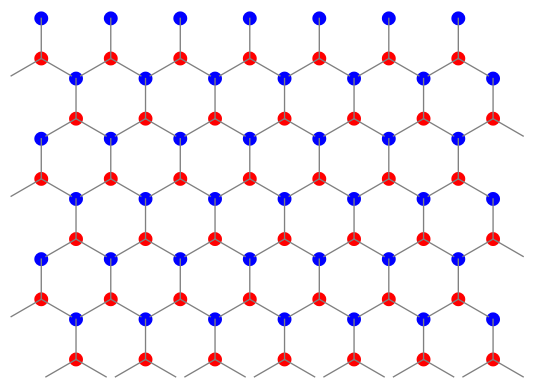
\includegraphics[width=4cm]{figures/introduction/graphene lattice.png}
	\end{subfigure}%
        \begin{subfigure}[c]{0.7\linewidth}
		\centering
		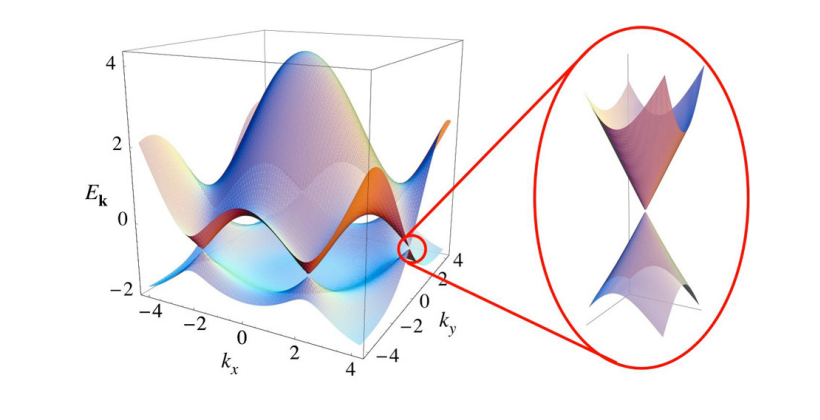
\includegraphics[width=\linewidth]{figures/introduction/bandstructure_graphene.png}
	\end{subfigure}%
	\caption{Left: Schematic hexagonal lattice of graphene showing carbon atoms in the A(red) and B(blue) sublattices. Right: Dispersion with zoom near the band-touching Dirac point (this panel taken from Ref.~\cite{neto2009electronic}).}
    \label{fig:schematiclatticegraphene}
    \end{figure}
    \begin{figure}
 	\centering
	\begin{subfigure}[c]{0.32\linewidth}
		\centering
		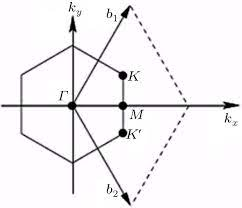
\includegraphics[width=\linewidth]{figures/introduction/brilluoinzonegraphene.png}
	\end{subfigure}
	\begin{subfigure}[c]{0.65\linewidth}
		\centering
		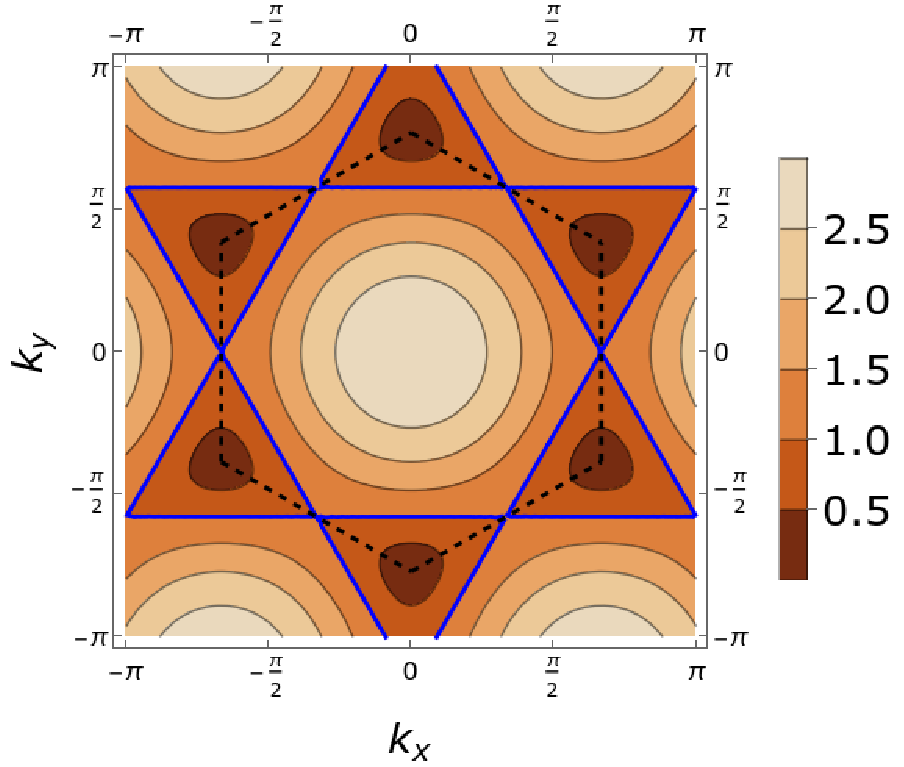
\includegraphics[width=\linewidth]{figures/introduction/graphenecontoursv2.pdf}
	\end{subfigure}
	\caption{Right: Energy contours of graphene showing the brilluoin zone in black dashed lines. The highlighted contour in blue is at the van Hove energy.  Left: The corresponding Brillouin zone marking the positions of the high symmetry points. (The left panel has been taken from Ref~\cite{neto2009electronic}).}
    \label{fig:Brillouin zone of graphene}
\end{figure}

The dispersion in Eq.~\eqref{eq:Graphene dispersion} shows interesting features at the $K, K^\prime$ and the $M$ points of the Brillouin zone( see Fig.~\ref{fig:schematiclatticegraphene}). 

\par
The $K$ point and its time reversed partner $K^\prime$ points are referred to as Dirac points. This is because the gap between the two bands closes at these points, and the dispersion is linear. Indeed, the low energy Hamiltonian close to for momenta $\vec{p}$ close to the $K$ point can be represented as 
\begin{align}
    H = v_F \,\Vec{p} \cdot \Vec{\sigma}.
    \label{eq:DiracHam}
\end{align}
\par 
The Dirac matrices in two dimensions are simply the $2x2$ Pauli matrices given by $\vec{\sigma}$. 
The corresponding dispersion $E(\Vec{p}) = v_F \abs{\vec{p}}$ is dubbed a Dirac cone, because it looks like a causal light cone from special relativity, just with an effective speed of light $v_F$. 

\par 
Graphene also has an interesting saddle-like dispersion near its $M$ point. This can be seen in Figs.\ref{fig:Brillouin zone of graphene} and \ref{fig:schematiclatticegraphene}. 
Since first derivatives vanish at a saddle point by definition, the dispersion is most faithfully captured by a Taylor expansion up to second order, with the expansion coefficients in the two principal directions having opposite sign: 
\begin{equation}
    E = E_v + \alpha p_x^2 -\beta p_y^2 \quad\quad \alpha,\beta>0, 
    \label{eq:dispQUAD}
\end{equation}
where $E_v$ is the energy at the saddle point, also known as the van Hove energy. Then, we can find the density of states: 
\begin{equation}
    \rho(E) = \int \frac{\dd p_y}{2\pi} \frac{\dd p_x}{2\pi} \, \delta(E - E_{\vec{p}})
    \label{eq:DOSformula}
\end{equation}
where we use the formula 
\begin{equation}
    \delta(g(x)) = \sum_i \frac{\delta(x-x_i)}{\abs{g^\prime(x_i)}}
\end{equation}
where $x_i$ are the roots of the function $g(x)$. Here we have $g(p_x) = E - E_v +\beta p_y^2 - \alpha p_x^2$, and $g^\prime(p_x) = -2\alpha p_x$. 
We obtain the roots of $g(p_x)$ as 
\begin{equation}
    p_x^\pm = \pm\sqrt{\frac{(E-E_v)+\beta p_y^2}{\alpha}}
\end{equation}
which gives, defining $\Tilde{E} = E - E_v$ 
\begin{equation}
    \rho(E) = \int \frac{\dd p_y}{2\pi} \int_{-\infty}^\infty \frac{\dd p_x}{2\pi} \, \frac{\delta(p_x - p_x^+) + \delta(p_x - p_x^-)}{2\sqrt{\alpha\beta}\sqrt{\frac{\Tilde{E}}{\beta} + p_y^2}}
\end{equation}

A note has to be made here about the range of $p_y$, which comes from the condition when $p_x$ has a solution, which is when $E - E_v + \beta p_y^2 > 0$. 

\begin{equation}
    \text{range of } p_y =
    \begin{cases} 
    \texttt{all}, \quad E>E_v \\
    p_y^2 > \abs{\frac{E-E_v}{\beta}}, \quad E<E_v
    \end{cases} 
\end{equation}

Introducing a cutoff for $p_y$ as $\Lambda$, for $E>E_v$, 
\begin{align}
    \rho(E) &= \frac{2}{\sqrt{\alpha\beta}} \int_0^\infty \frac{\dd p_y}{(2\pi)^2} \frac{1}{\sqrt{\frac{\Tilde{E}}{\beta} +  p_y^2}} \nonumber \\
    &= \frac{1}{2\pi^2\sqrt{\alpha\beta}} \log\abs{\frac{2\Lambda\sqrt{\beta}}{\sqrt{E - E_v}}} \nonumber \\
    &= \frac{1}{4\pi^2 \sqrt{\alpha\beta}} \log\abs{\frac{\Tilde{\Lambda}}{E - E_v}}
    \label{eq:LOGvHSDoS}
\end{align}
with $\Tilde{\Lambda} = 4\Lambda^2\beta$. The density of states is symmetric about the van Hove energy, and we obtain exactly the same expression for $E<E_v$.  


\section{The concept of a higher order van Hove singularity} 
The hyperbolic geometry of the Fermi surface near the van hove energy and its enhanced density of states can be understood quite intuitively by means of Fig.~\ref{fig:logcontours}. Much like the SYK model, the enhanced DoS is not from a degeneracy, but the ability to pack energy levels densely close together at low energy. More and more states can be fit into the corner created by the touching Fermi surfaces at the van hove energy, leading to the diverging density of states.
\begin{figure}[h]
    \centering
    \begin{subfigure}[t]{0.45\linewidth}
        \centering
        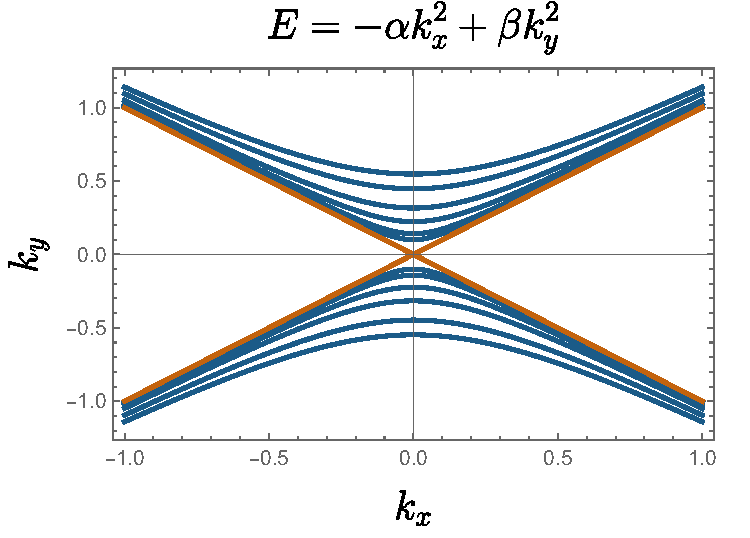
\includegraphics[width=\textwidth]{figures/introduction/logcontours.pdf}
        \caption{\centering conventional van Hove singularity, Eq.~\eqref{eq:dispQUAD}}
        \label{fig:logcontours}
    \end{subfigure}
    \hfill
    \begin{subfigure}[t]{0.45\linewidth}
        \centering
        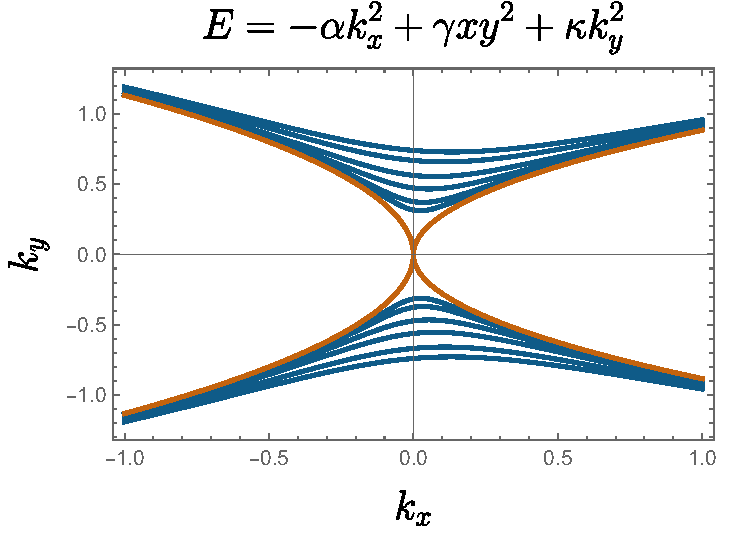
\includegraphics[width=\textwidth]{figures/introduction/paracontours.pdf}
        \caption{\centering higher order van hove singularity}
        \label{fig:paracontours}
    \end{subfigure}
    \hfill
    \caption{Hyperbolic geometry of the energy contours near a van Hove singularity. In each case, the limiting curve for $E=0$, which is here the van Hove energy, is shown by an orange line.}
    \label{fig:vanHoveillustration}
\end{figure}

\par 
Near a conventional logarithmic van hove singularity, the contours of equal energy form hyperbolae in momentum space. This is easily visible in the topology change of the Fermi surface, as it crosses the van hove energy. At exactly the van hove energy, the Fermi surface is made of the asymptotes of the hyperbola, which are two lines meeting at a point. This can be generalized in many ways, the most obvious of which is to have a Fermi surface composed of the intersection of two parabolae with a quartic dispersion(see Fig. ~\ref{fig:paracontours}). This also has a direct effect in the type of singularity in the density of states: in this case being a power law $\rho(E)\sim\abs{E}^{\nicefrac{-1}{4}}$~\cite{Yuan2019,Yuan2020PRB-classification}. These can be neatly classified by a recently developed catastrophe theory formalism~\cite{chandrasekaran2020catastrophe,zakharov2024landau,classen2024high}.  
\par
The higher order van hove singularity appears in many physical systems, such as the cuprates~\cite{markiewicz1989correlation,markiewicz2023investigating,paul2023exceptional}, in twisted bilayer graphene and other transition metal dichalcogenide bilayers.
The difference however between the cuprates and monolayer graphene as compared to the moire materials is that, while in monolayer graphene and the cuprates the van hove singularity (higher order or otherwise) is far away from the Fermi energy (eV scale) meaning that they are relatively difficult to reach in experiments, whereas they are close to the Fermi energy (meV scale) in the moire materials. Accordingly, they will also have strong effects on measurable properties, as we shall see in the next section.
%
\section{Enhanced interactions near van hove points - towards Twisted Bilayer graphene}
%
Graphene is known to not be superconducting at charge neutrality owing to it being a bad metal~\cite{efetov2014towards}, i.e having a low density of states at the Dirac point. This can be understood in the following cartoon like picture. Assuming, BCS theory of superconductivity holds, the superconducting transition temperature is obtained by solving the linearized gap equation to be 
\begin{equation}
    T_c = \omega_0 \exp{-\frac{1}{g\rho(E_F)}},
    \label{eq:BCSTc}
\end{equation}
where $g$ is a parameter characterizing electron-electron attraction, $\omega_0$ is a UV cutoff (usually taken to be the Debye frequency) and $\rho(E_F)$ is the density of states at the Fermi energy. The vanishing density of states of the Dirac cone implies an negative infinity in the exponential in Eq.~\eqref{eq:BCSTc}, meaning no superconductivity at any finite temperature.

\par
Thus it came as a surprise when twisted bilayer graphene was observed to be superconducting in some recent landmark experiments~\cite{Cao2018,Caocorrelated2018,oh2021evidence,lisi2021observation}. But we will argue here that with the considerations of the enhanced DoS coming from the van hove singularity, now quite close to the Fermi level, that it should not be so surprising at all. 

\par
This is a part of a general phenomenon in which interactions get enhanced by the hyperbolic geometry in the Fermi surface. A rigorous argument for breakdown of Fermi liquid theory has been addressed in the seminal works of Shankar and Polchinksi in Refs.~\cite{shankar1991renormalization,shankar1994renormalization,polchinski1992effective} by considering the renormalization effects of interactions upon scaling momenta in the low energy effective theory towards the Fermi surface, but we shall sketch a caricature of it below that captures the essence of the argument without all of its sophisticated machinery. 

\begin{figure}[h!]
    \centering
    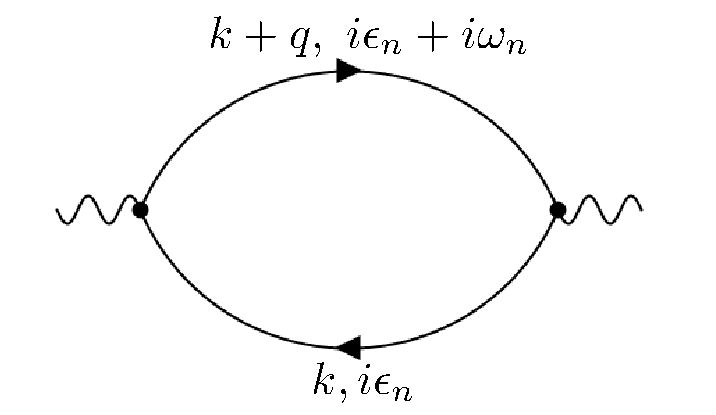
\includegraphics[width=0.8\linewidth]{figures/introduction/LabeledChiQOmdiagramv2.pdf}
    \caption{Polarization bubble diagram $\Pi(q,i\omega_n)$: This shows up in charge susceptibility, self energy due to fermion-fermion interactions, phonon self energy among others}
    \label{fig:PHbubblediagram}
\end{figure}
Consider the particle-hole bubble shown in Fig.~\ref{fig:PHbubblediagram}. This diagram - the polarization bubble - arises in many different contexts. In linear response theory, this is the leading diagram corresponding to the charge susceptibility $\chi(q,i\omega_n)$, and is related to the dielectric constant~\cite{coleman2015introduction}. Another context where it can appear is as a sub-diagram in the leading contribution to decay of quasiparticles in the self energy of an interacting Fermi gas ~\cite{Sachdev_2011}, where the full self energy is
\begin{equation}
\Sigma(k,\epsilon_n) = g^2\int d\vec{q} \,T\sum_{\omega_n}\Pi(\vec{q},\omega_n)G_0(\vec{k}+\vec{q},i\epsilon_n + i\omega_n), 
\end{equation}
and $g$ is the simplified contact interaction coefficient in Eq.~\eqref{eq:schemHam}.

\par
The evaluation of the bubble diagram gives us: 
\begin{align}
    \chi_0(q,i\omega_n) = T\sum_{\epsilon_n} \int d\vec{k}\, G^0(k+q,\epsilon_n+\omega_n)G^0(k,\epsilon_n) 
\end{align}
We can first study the long wavelength static limit $q\xrightarrow{}0, \omega_n = 0$. Then, 
\begin{align}
    \chi_0(q\xrightarrow{}0, \omega_n = 0) &= T\sum_{\epsilon_n} \int d\vec{k}\, G^0(k,\epsilon_n)G^0(k,\epsilon_n) \nonumber \\
    &= \int d\vec{k} \left[T\sum_{\epsilon_n}\left(\frac{1}{i\epsilon_n - E_{\vec{k}}}\right)^2\right].
\end{align}
This contour integral is trivial to do if one remembers that 
\begin{equation}
    T\sum_{\epsilon_n} \frac{1}{i\epsilon_n-E_k} = n_F(E_k)\,,
\end{equation}
with $n_F(E)$ being the Fermi-Dirac function. Then we see that 
\begin{align}
    \chi_0(q\xrightarrow{}0, \omega_n = 0) &= \int d\vec{k}\, \dv{E_k}( n_F(E_k)) \\ 
    &= -\int d\vec{k} \, \delta(E_k - E_F) = -\rho(E_F)\,.
\end{align}
We have used also that at zero temperature, 
\begin{equation}
    \dv{E_k}( n_F(E_k)) = -\delta(E_k - E_F)\,.
\end{equation}
It's straightforward to generalize to the case of finite $q$ as well using the partial fractions trick: 
\begin{align}
    \chi_0(q, \omega_n = 0) &= T\sum_{\epsilon_n} \int d\vec{k}\, G^0(k+q,\epsilon_n)G^0(k,\epsilon_n) \,,\nonumber \\ 
    &= \int d\vec{k}\, T\sum_{\epsilon_n} \frac{1}{i\epsilon_n - \epsilon_{k+q}} \cdot \frac{1}{i\epsilon_n - \epsilon_k} \,, \nonumber \\
    &= \int d\vec{k}\, \frac{1}{\epsilon_{k+q} - \epsilon_k}\, T\sum_{\epsilon_n} \left(\frac{1}{i\epsilon_n - \epsilon_{k+q}} -  \frac{1}{i\epsilon_n - \epsilon_k} \right)\,,\nonumber \\
    &= \int \frac{d^d k}{(2\pi)^d} \frac{n_F(\epsilon_{k+q}) - n_F(\epsilon_k)}{\epsilon_{k+q}-\epsilon_{k}} \,.
\end{align}

 For the $k^2$ dispersions in 1,2 and 3 dimensions, it is also possible to evaluate these integrals exactly in the static response limit (i.e. at $\omega$ = 0)~\cite{mihaila2011lindhard}, and we present just the result below: 
\begin{enumerate}
    \item The susceptibility is a constant in the limit of vanishing wave-vector: i.e. a very slowly spatially varying external field. \begin{equation}
        \chi_0(q\xrightarrow{}0,\omega=0) = -\rho(\epsilon_F)\,.
    \end{equation}
    \item For finite q, there is a log-singularity at $q=2k_F$ in the susceptibility, which is a branch cut in the complex plane. \begin{align}
        \chi_0(q,\omega=0) &= -\rho(\epsilon_F) F(\frac{q}{2k_F}) \,\,,\\
        F(x) &= \frac{1}{2} + \frac{1-x^2}{4x} \log\abs{\frac{1+x}{1-x}}   
    \end{align}
\end{enumerate}

\par
Thus one can clearly see the vital effect the density of states has on the interaction corrections to the Fermi gas. In a high carrier density metal in three dimensions like bulk copper, $\rho(E_F)$ can be taken to be more or less a constant, and weak interactions can be treated perturbatively to just give small corrections to the non-interacting theory. However, when the Fermi energy is close to a van-Hove singularity, the divergence in the density of states makes the effective interaction strength large, leading to instabilities and the breakdown of quasiparticles and Fermi liquid theory.

\par
We have spelled out the calculation of the charge susceptibility which arises from the particle-hole bubble in Fig.~\ref{fig:PHbubblediagram}, but the exact same enhancement effect from the density of states at the Fermi level also shows up in other physical effects, such as in spin-spin correlation functions, or in the particle-particle bubble for the susceptibility towards pairing in the theory of superconductivity~\cite{Classen2020PRB}. 

\par
Having understood the crucial role that van Hove points can play in enhancing correlations between electrons, we will argue that both conventional and more exotic higher order van Hove singularities play an important role in the twisted bilayer graphene (TBG). 
\par
As the name suggests, twisted bilayer graphene is made of two layers of mono layer graphene, at a relative angle to each other. The relative misalignment between the layers originating from the twist leads to the formation of a Moire pattern. 
\begin{figure}
    \centering
    \begin{subfigure}[t]{0.45\linewidth}
        \centering
        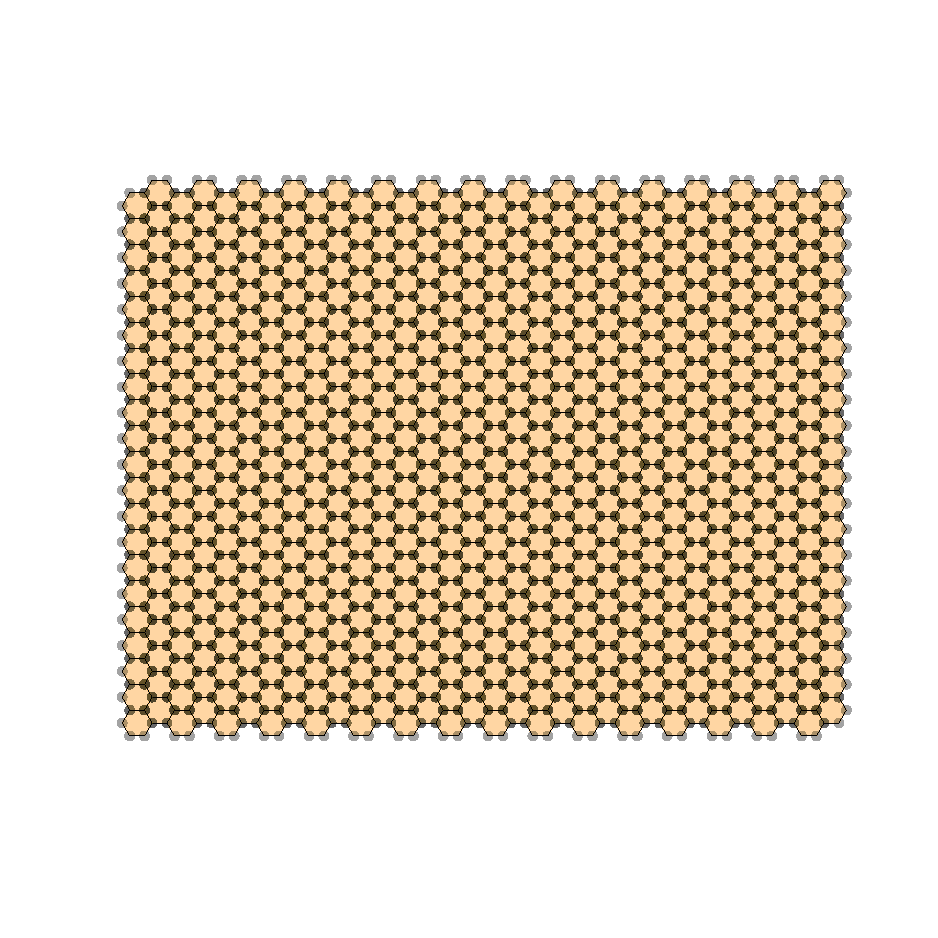
\includegraphics[width=\linewidth]{figures/introduction/zeroTwist.pdf}
        \caption{\centering Untwisted AA stacked graphene bilayer}
        \label{fig:untwisted}
    \end{subfigure}
    \begin{subfigure}[t]{0.45\linewidth}
        \centering
        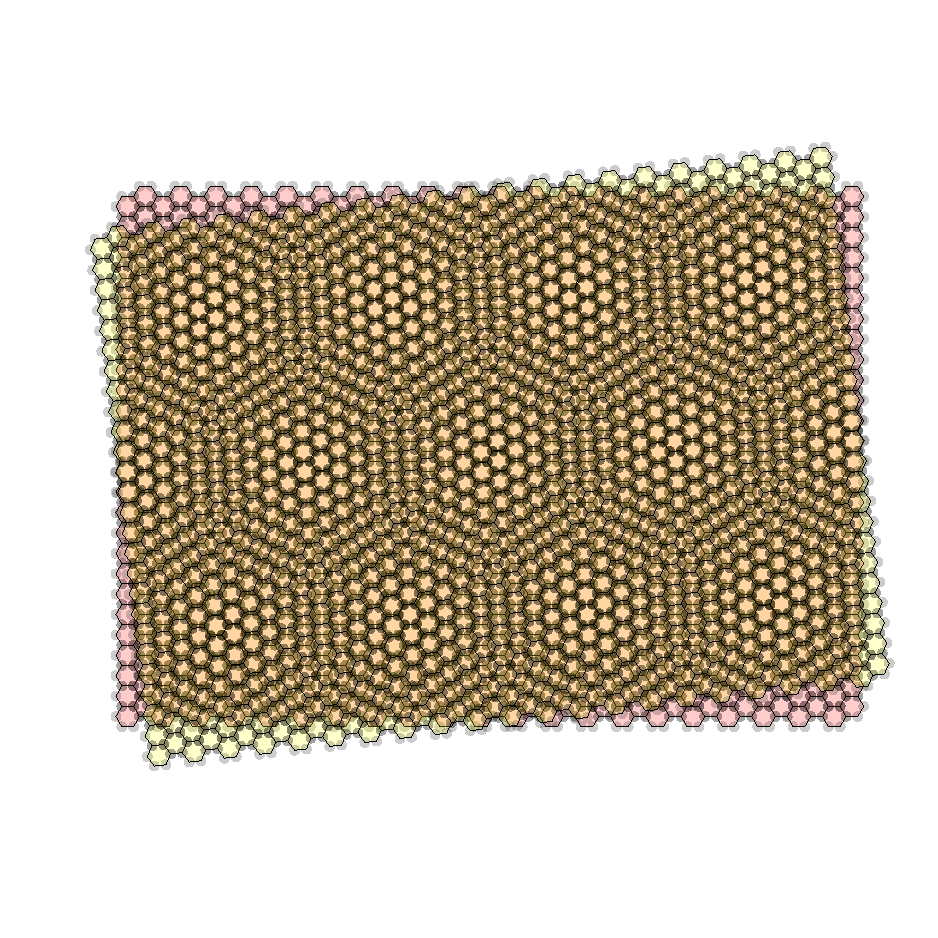
\includegraphics[width=\linewidth]{figures/introduction/6_40Moire.pdf}
        \caption{\centering Relative twist of $6.40^\circ$ with $2892$ atoms in the unit cell.}
        \label{fig:twisted}
    \end{subfigure}
    \caption{Moire pattern in twisted bilayer graphene. Large twist angle shown for ease of illustration. In realistic samples, much smaller twists under $2^\circ$ are seen, with up to $\sim 10000$ carbon atoms in the unit cell at the magic angle. (Image generated using the Wolfram demonstrations project~\cite{MoireWolfram}).}
    \label{fig:MoirePattern}
\end{figure}

The Moire pattern forms a larger superlattice as is easily visible in Fig.~\ref{fig:untwisted}. From simple geometric arguments, the lattice constant for the Moire superlattice can be expressed in terms of the lattice constant of graphene for a twist angle $\theta$ as~\cite{Bistritzer2011}
\begin{align}
    L_\theta &= \frac{\sqrt{3}a}{2\sin\left(\frac{\theta}{2}\right)}\, \nonumber  \\
    &\approx \frac{\sqrt{3}a}{\theta} \quad\quad, \text{for small twist angles.}
\end{align}
Consequently, the gigantic real space superlattice implies a tiny reciprocal lattice, dubbed the Moire (or mini) Brillouin zone (MBZ).  
This fact has a far reaching consequence for the low energy band structure of TBG, shown in pictorially in Fig.~\ref{fig:bandflattening}. 
\begin{figure}[!ht]
    \centering
    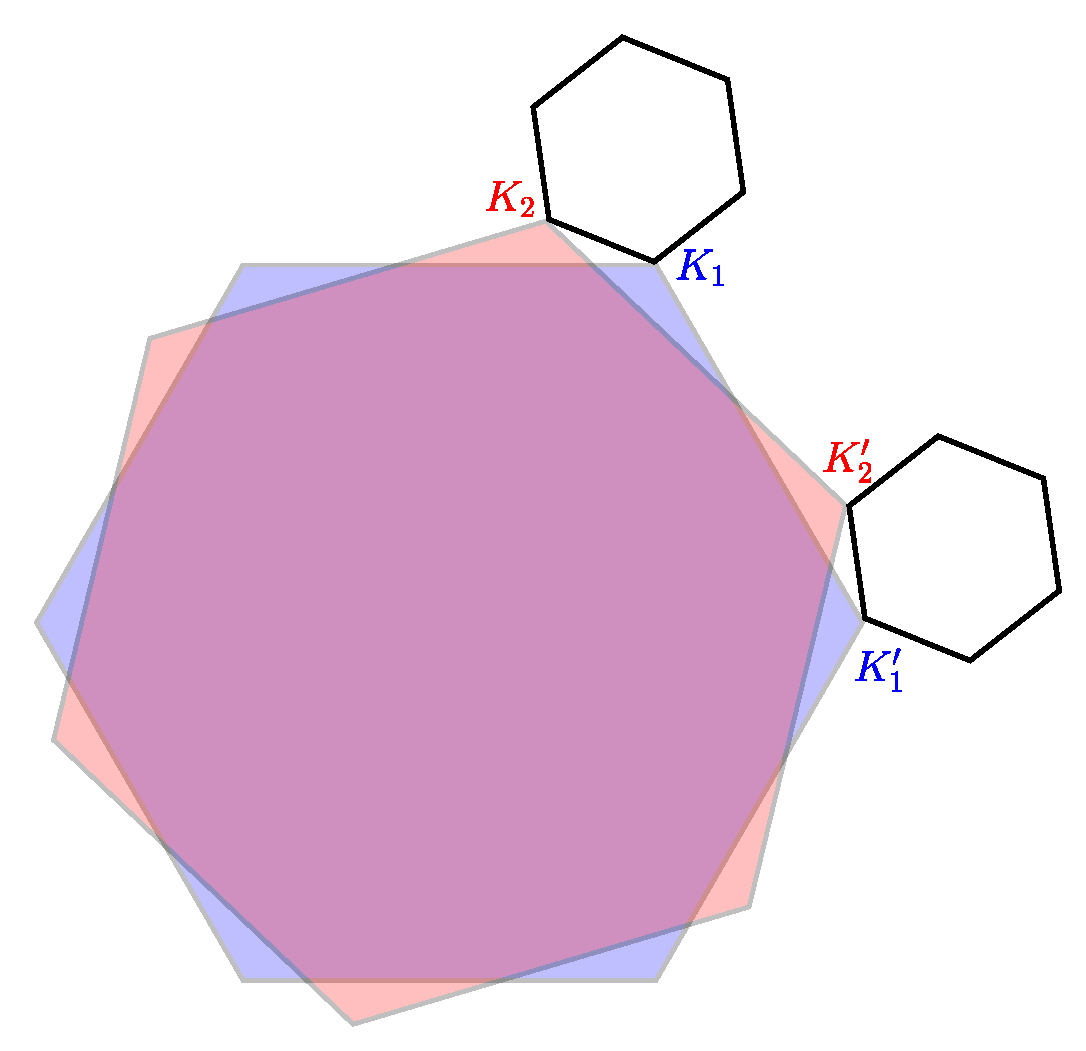
\includegraphics[width=0.5\linewidth]{figures/introduction/TBGmoire.pdf}  
    \caption{Illustration of the formation of the Moire Brillouin zone. Starting from AA stacking, one layer is rotated relative to the other layer by a small angle. It is easy to see from this figure that if $\vec{k}$ was the wavevector of the K point of the Brillouin zone of monolayer graphene, then the size of the mini Brillouin zone is $k\theta$.}
    \label{fig:moirebrilluoinzone}
\end{figure}
\par
Since the moire lattice is also hexagonal, it must also have an effective Dirac cone in its spectrum. 
If we restrict our attention only to the low energy bands, we can look simply at what happens to the Dirac cone at the K and K${}^\prime$ points of each individual monolayer. These form the corners of the MBZ. The smallness of the MBZ means that there will be significant overlap in the two lowest energy bands, and the hybridization caused by the interlayer hopping will lead to a level repulsion, similar to the formation of the bonding and antibonding orbitals in molecular orbital theory description of the hydrogen molecule. This is shown pictorially in Fig.~\ref{fig:bandflattening}.

\begin{figure}[!ht]
    \centering
    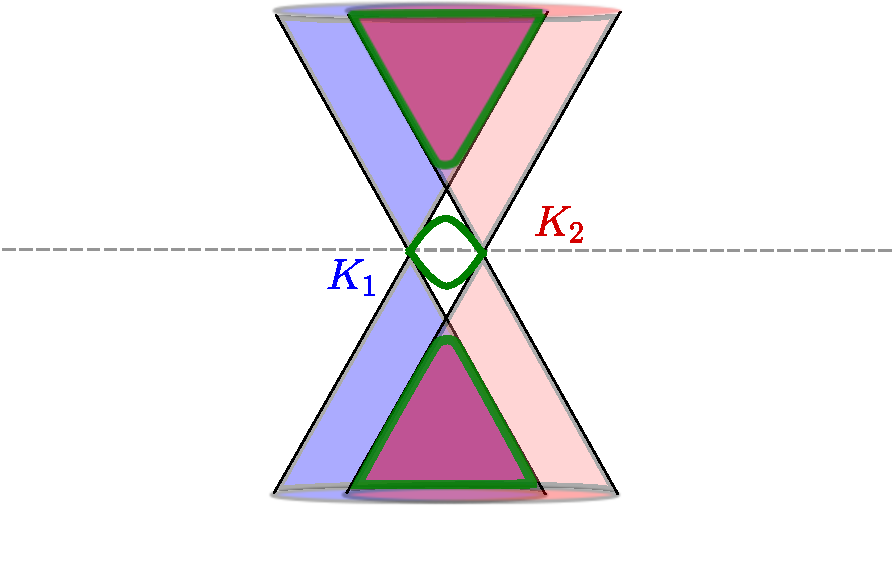
\includegraphics[width=0.5\linewidth]{figures/introduction/BandFlattening.pdf}
    \caption{Illustration of the formation of the flat bands: When the two Dirac cones from each layer are close together, there's a significant overlap in their wavefunction, and hybridization effects can be large enough to render the bottom band almost completely flat.}
    \label{fig:bandflattening}
\end{figure}
\par
This simple effective continuum model was first described by Bistritzer and Macdonald in their seminal work in Ref.~\cite{Bistritzer2011}. Their key finding was that at some "magic" angle, the bonding orbital thus formed experiences such a degree of energy lowering that the lowest band becomes almost completely flat. For twisted bilayer graphene, this angle is roughly $1.05^\circ$. In other words, this is the angle at which the effective Dirac velocity of the cone corresponding to hexagonal lattice of the bilayer system vanishes. 
\par
Furthermore, the flat band thus formed for small twist angles is not completely flat, but has features at the scale of meV, including van Hove singularities. Unlike the case of the square lattice or mono layer graphene, which have vHS at high energies in the eV scale, these low energy vHs in TBG are very close to the Fermi level, and will play an important role in the low energy physics of the material. At exactly the magic angle, we even observe a higher order vHS, and the role it plays in the ability of the system to screen the spin of magnetic impurities will be the subject of Chapter~\ref{ch:KondoTBG}.

















\section{This thesis}
In the introduction, we have explored two very different electronic systems, and uncovered clandestine hyperbolic geometries in each of them.  

\subsection{Chapter 1 - The Kondo effect in Twisted bilayer graphene}
This chapter concerns the fate of dilute magnetic impurities embedded in twisted bilayer graphene. The density of states profile of twisted bilayer graphene has both a dirac cone and a van Hove singularity in it, the location of which moves closer towards the Fermi energy upon changing the twist angle between the layers closer and closer to $1.05^\circ$. In a metal with a constant density of states and a large carrier density, the magnetic moment of the impurity gets strongly screened by the conduction electrons in a phenomenon called the Kondo effect for temperatures below a characteristic scale called the Kondo temperature. This is not seen in monolayer graphene owing to the low density of states of the Dirac cone in similar spirit to Eq.~\ref{eq:BCSTc}. The chapter first addresses the modeling of the low energy band structure of twisted graphene using the continuum Bistritzer-MacDonald model~\cite{Bistritzer2011}, presents a method to accurately determine the positions and nature of the van Hove singularities close to the Fermi level, and then presents numerical renormalization group results for the impurity entropy and spectral function at finite temperature for this version of the Kondo problem. The key prediction is a revival of the Kondo effect at the lowest energy scales at exactly the magic angle of twisted bilayer graphene. The results of this chapter have been published in Ref.~\cite{shankar2023kondo} and further studies confirming the prediction using more sophisticated models have appeared from other groups since in Ref.~\cite{chang2023vacancy}. 

\subsection{Chapter 2 - Chaos in the bipartite Sachdev-Ye-Kitaev model}
This chapter studies the scrambling dynamics of the b-SYK model by calculation of its Lyapunov exponent, both in the fully conformal limit and at intermediate and weak coupling as the population ratios of the A and B Majoranas are changed. The population imbalance endows the A and B Majoranas with separate conformal dimensions, but the analysis presented determines the model as a whole to have one unique exponent. This is understood in terms of scattering pathways of the A and the B Majoranas mixing with each other and the model always picking the scattering pathway with the fastest rate. Furthermore, although the model saturates the chaos bound presented in the seminal work of Ref.~\cite{maldacena_bound_2016} in the conformal limit, it was observed that even the corrections to the Lyapunov exponent at intermediate coupling in the b-SYK model is uninfluenced by perturbations to the conformal dimension of the A and B fermions, which is a surprising result. This chapter has been published in Ref.~\cite{shankar2023lyapunov}.


\subsection{Chapter 3 - Wormholes in the Yukawa-Sachdev-Ye-Kitaev model}
In this chapter, we study a model of two YSYK dots coupled with a tunneling interaction $\lambda$. In the weak tunneling limit, the quantum state of the system is well approximated by the thermo-field double (TFD) state. This makes the system dual to an eternal traversable wormhole, along the lines of Ref.~\cite{maldacena2018eternal,maldacena2003eternal}. In the TRS broken non-superconducting state, we indeed find a first order transition of the system from the two black holes phase to a wormhole phase, with a clear signature in the scaling of the boson and fermion Green's functions. Furthermore, we find that the wormhole phase survives the competition from superconducting order, which arises upon the restoration of TRS. On the gravitational side, superconductivity is described by scalar hair. Our key finding is that the system in the superconducting state remains a traversable wormhole for the fermionic excitations, but not for the scalar hair. Additionally, since the system on the field theory side represents two coupled superconductors, we investigate the Josephson effect that arises from twisting the phase of the two sides relative to one another. This chapter is still a manuscript under preparation. 